\cotefile{36}

\scanpage{44}
\uline{Foncteurs adjoints}

\uline{Definition 1} soient $X,Y\in(\mathrm{Cat})$, $f:X\longrightarrow Y$ et $g:Y\longrightarrow X$, on dit que $(f,g)$ est un couple de foncteurs adjoints, ou que $g$ est adjoint de $f$, ou que $f$ est coadjoint de $g$, s'il existe un

\deleted{$\unsure{\forall}$}

\[
\begin{gathered}
\mathcal H^1(X,\underline{\operatorname{Hom}}(\gamma,G))\simeq\\
\mathcal H^1(X,\underline{\operatorname{Ext}}^1(\gamma,G))
\end{gathered}
\]
\[\operatorname{Ext}^1(\gamma,\]

\figure{\begin{tikzpicture}[x=1cm,y=1cm]
\draw[line width=.6pt] (0,.16) .. controls (.9,.22) and (2,.04) .. (3.18,0);
\draw[line width=.6pt] (.02,-.12)--(3.18,0);
\draw[line width=.45pt] (3.23,-.01)--(6.14,4.00);
\draw[line width=.55pt] (6.29,4.10) .. controls (7.3,4.10) and (9.0,3.94) .. (10.05,3.94);
\end{tikzpicture}}

\[X\longrightarrow\underline{\operatorname{Hom}}_{S\text{-gr}}(\gamma,G)\]
\[X\times\gamma\longrightarrow G\]
\diagram{\begin{tikzcd}[ampersand replacement=\&,row sep=large]
\deleted{\unsure{\gamma}}\ \gamma\arrow[r]\arrow[dr,no head,shorten <=12pt,shorten >=5pt]\&\underline{\operatorname{Hom}}_S(X,G)\\
S\&\overset{\unsure{p_2|\mathrm{pr}_2|\Pi_2}}{\unsure{C|G}}
\end{tikzcd}}
\[\operatorname{Hom}(\gamma,\]

\[
\begin{array}{l}
\displaystyle\prod^{\circ}_{X/S}\gamma_X\\[3pt]
\quad\Vert\\[3pt]
\underline{\operatorname{Hom}}_S(X,\gamma)\doteq\gamma
\end{array}
\]

\diagram{\begin{tikzcd}[ampersand replacement=\&,column sep=small]
e\arrow[r]\&\gamma\arrow[r]\&\underline{\operatorname{Hom}}_S\unsure{(|U}X,\gamma)\arrow[r]\&\operatorname{Hom}(X,a;\gamma)\arrow[r]\&0
\end{tikzcd}}

\figure{\begin{tikzpicture}\draw (0,0)--(.35,.12);\end{tikzpicture}}
\margin{43}

\scanpage{45}
D'après le théor. d'Artin--Schreier--Witt, on a
\[
H^1(A,\mathbb Z/p)\simeq H^1(A,\underline O_A)^{\unsure{(\varphi)|(p)}}_{\deleted{\unsure{\varphi}}}
\]
éléments de $H^1(A,\underline O_A)$ tels que
\[Fx=x\]
\[
H^1(A,\mathbb Z/p^n)\simeq H^1(A,\underline O_A(W_n))^{\unsure{(\varphi)|(p)}}
\]
--- $H^1(A,\underline O_A(W_n))$ tels que
\[Fx=x\]
\[
\vcenter{\hbox{\begingroup
\setbox0=\hbox{$\displaystyle \operatorname{Hom}(\pi_1^p(A),\mathbb Z_p)\simeq H^1(A,\deleted{\unsure{\mathbb Q_p}}\mathbb Z_p)\simeq H^1(A,\mathbb W)^{\unsure{(\varphi)|(p)}}_{\deleted{\unsure{\varphi}}}$}
\dimen0=\wd0 \advance\dimen0 by 18pt
\dimen2=\ht0 \advance\dimen2 by \dp0 \advance\dimen2 by 16pt
\rlap{\raisebox{\dimexpr-\dp0-8pt\relax}{%
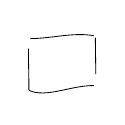
\begin{tikzpicture}[x={\dimexpr\dimen0/1020\relax},y={\dimexpr-\dimen2/145\relax},line width=.3pt]
\path[use as bounding box] (0,0) rectangle (1020,145);
\draw (40,23) .. controls (350,23) and (680,9) .. (982,17);
\draw (12,44) .. controls (11,77) and (20,110) .. (18,132);
\draw (21,132) .. controls (270,149) and (650,121) .. (981,122);
\draw (1002,21) -- (1009,98);
\end{tikzpicture}}}%
\kern9pt\box0\kern9pt\endgroup}}
\]
\deleted{\unsure{on}} \inserted{d'où} \deleted{\inserted{\unsure{a}}} on déduit un \deleted{accouplement} isomorphisme
\[
\vcenter{\hbox{\begingroup
\setbox0=\hbox{$\displaystyle \deleted{\pi_1^p(A)\times H^1(A,\mathbb W)_s\longrightarrow\mathbb Z_p}$}
\dimen0=\wd0 \advance\dimen0 by 18pt
\dimen2=\ht0 \advance\dimen2 by \dp0 \advance\dimen2 by 16pt
\rlap{\raisebox{\dimexpr-\dp0-8pt\relax}{%
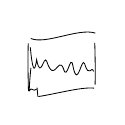
\begin{tikzpicture}[x={\dimexpr\dimen0/770\relax},y={\dimexpr-\dimen2/140\relax},line width=.3pt]
\path[use as bounding box] (0,0) rectangle (770,140);
\draw (35,22) .. controls (200,35) and (570,0) .. (756,11);
\draw (6,32) .. controls (2,63) and (4,103) .. (9,129);
\draw (120,140) .. controls (310,135) and (600,120) .. (744,123);
\draw (750,31) .. controls (756,65) and (756,95) .. (754,116);
\draw (30,40) .. controls (48,79) and (75,99) .. (100,65) .. controls (145,108) and (180,54) .. (212,68) .. controls (300,116) and (340,56) .. (400,83) .. controls (440,112) and (478,50) .. (505,77) .. controls (559,128) and (600,58) .. (636,73) .. controls (690,105) and (710,75) .. (737,89);
\draw (36,82) .. controls (25,101) and (15,126) .. (19,128) .. controls (45,119) and (60,132) .. (100,125);
\draw (105,122) -- (114,140);
\end{tikzpicture}}}%
\kern9pt\box0\kern9pt\endgroup}}
\]
\[
\vcenter{\hbox{\begingroup
\setbox0=\hbox{$\displaystyle \deleted{\operatorname{Hom}_{\mathrm{cont}}(\pi_1^p(A),\Lambda)\simeq H^1(A,\mathbb W)_s}$}
\dimen0=\wd0 \advance\dimen0 by 18pt
\dimen2=\ht0 \advance\dimen2 by \dp0 \advance\dimen2 by 16pt
\rlap{\raisebox{\dimexpr-\dp0-8pt\relax}{%
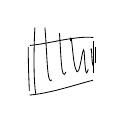
\begin{tikzpicture}[x={\dimexpr\dimen0/900\relax},y={\dimexpr-\dimen2/190\relax},line width=.3pt]
\path[use as bounding box] (0,0) rectangle (900,190);
\draw (29,49) .. controls (260,45) and (620,22) .. (858,27);
\draw (8,53) .. controls (7,103) and (16,145) .. (22,174);
\draw (24,186) .. controls (300,181) and (630,157) .. (853,145);
\draw (858,37) -- (858,126);
\draw (880,53) -- (880,97);
\draw (94,0) .. controls (79,61) and (76,148) .. (106,183);
\draw (225,0) .. controls (258,76) and (250,163) .. (318,144);
\draw (415,15) .. controls (437,74) and (437,153) .. (500,122);
\draw (558,37) .. controls (575,0) and (585,95) .. (630,115) .. controls (680,149) and (720,37) .. (738,66) .. controls (750,105) and (756,143) .. (791,115);
\draw (824,62) .. controls (842,46) and (832,99) .. (856,105);
\end{tikzpicture}}}%
\kern9pt\box0\kern9pt\endgroup}}
\]
qui est une dualité \deleted{\unsure{de}} de $\mathbb Z_p$-modules libres de type fini

D'autre part, utilisant encore le fait que tout revêtement de $A$ est une variété abélienne, on trouve aussi
\[\boxed{\pi_1^p(A)\simeq T_p(A)}\]
d'où en les composant
\[
\vcenter{\hbox{\begingroup
\setbox0=\hbox{$\displaystyle T_p(A)\times H^1(A,\mathbb W)^{\unsure{(\varphi)|(p)}}\longrightarrow\mathbb Z_p$}
\dimen0=\wd0 \advance\dimen0 by 18pt
\dimen2=\ht0 \advance\dimen2 by \dp0 \advance\dimen2 by 16pt
\rlap{\raisebox{\dimexpr-\dp0-8pt\relax}{%
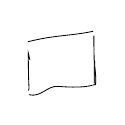
\begin{tikzpicture}[x={\dimexpr\dimen0/795\relax},y={\dimexpr-\dimen2/190\relax},line width=.3pt]
\path[use as bounding box] (0,0) rectangle (795,190);
\draw (0,39) .. controls (310,20) and (500,23) .. (755,10);
\draw (25,89) -- (7,70) .. controls (8,106) and (8,135) .. (16,168) -- (8,173);
\draw (13,185) .. controls (160,193) and (220,160) .. (350,162) .. controls (510,165) and (650,165) .. (748,159);
\draw (764,22) .. controls (763,60) and (771,85) .. (768,153);
\draw (773,91) .. controls (775,122) and (778,145) .. (779,157) -- (754,158);
\draw (774,107) .. controls (789,134) and (787,147) .. (784,157) -- (778,158);
\end{tikzpicture}}}%
\kern9pt\box0\kern9pt\endgroup}}
\]
qui est une dualité de $\mathbb Z_p$-modules libres de type fini.

\deleted{qu'on peut aussi écrire} \unsure{donc|d'où} on déduit
\[
\vcenter{\hbox{\begingroup
\setbox0=\hbox{$\displaystyle \operatorname{Hom}_{\mathrm{cont}}(T_p(A),\deleted{\unsure{\mathbb Z_\ell|\Lambda}}W_\infty(k))\simeq H^1(A,\mathbb W)_s$}
\dimen0=\wd0 \advance\dimen0 by 18pt
\dimen2=\ht0 \advance\dimen2 by \dp0 \advance\dimen2 by 16pt
\rlap{\raisebox{\dimexpr-\dp0-8pt\relax}{%
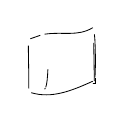
\begin{tikzpicture}[x={\dimexpr\dimen0/910\relax},y={\dimexpr-\dimen2/180\relax},line width=.3pt]
\path[use as bounding box] (0,0) rectangle (910,180);
\draw (35,29) -- (166,20);
\draw (224,17) .. controls (470,10) and (660,24) .. (861,0);
\draw (9,47) .. controls (10,91) and (18,133) .. (14,159);
\draw (47,170) .. controls (320,186) and (580,165) .. (860,140);
\draw (873,40) -- (881,140);
\draw (879,20) .. controls (887,7) and (904,88) .. (889,130);
\draw (861,146) -- (895,146) -- (896,132);
\draw (224,161) -- (233,158);
\draw (239,156) .. controls (254,148) and (263,130) .. (267,109);
\end{tikzpicture}}}%
\kern9pt\box0\kern9pt\endgroup}}
\]
\margin{44}

\scanpage{46}
$A$ variété abélienne en. car $p$. On a, pour la partie de $\pi_1(A)$ première à $p$
\[
\pi_1^{\neq p}(A)\simeq\varprojlim_{\substack{n\\\text{arith}\\(n,p)=1}}\deleted{\unsure{n}}A^{(n)}
\]
où $\deleted{\unsure{n}}A^{(n)}$ est le noyau de $A\xrightarrow{n}A$, et où $A^{(mn)}\mathbin{-}A^{(n)}$ est la multiplication par $m$.
\[
\vcenter{\hbox{\begingroup
\setbox0=\hbox{$\displaystyle \pi_1^\ell(A)\simeq\varprojlim_{\deleted{\unsure{\ell}}k} A^{(\ell^k)}\simeq T_\ell(A)=\operatorname{Hom}(\underline{\mathbb Q}_\ell/\mathbb Z_\ell,A)$}
\dimen0=\wd0 \advance\dimen0 by 18pt
\dimen2=\ht0 \advance\dimen2 by \dp0 \advance\dimen2 by 16pt
\rlap{\raisebox{\dimexpr-\dp0-8pt\relax}{%
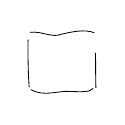
\begin{tikzpicture}[x={\dimexpr\dimen0/1256\relax},y={\dimexpr-\dimen2/177\relax},line width=.3pt]
\path[use as bounding box] (0,0) rectangle (1256,177);
\draw (41,12) .. controls (250,8) and (450,27) .. (610,17) .. controls (800,11) and (1030,3) .. (1217,13);
\draw (8,31) .. controls (2,63) and (8,116) .. (27,153);
\draw (58,159) .. controls (310,179) and (545,161) .. (785,164) .. controls (975,165) and (1155,166) .. (1192,156);
\draw (1235,65) .. controls (1243,78) and (1236,116) .. (1245,155);
\end{tikzpicture}}}%
\kern9pt\box0\kern9pt\endgroup}}
\]
\margin{module de Tate}
$\ell$ étant un nb premier $\neq p$. Ce résultat provient du fait qu'un \uline{revêtement non ramifié d'une variété abélienne est une variété abélienne}

D'après Kummer, on a d'autre part
\[
\deleted{\text{\unsure{Dual|Donc}}}\operatorname{Hom}(\pi_1^\ell(A),U_\ell)\simeq
\text{sous-gpe de }\unsure{\mathfrak P|\mathfrak D}(A)=H^1(A,\underline O_{\unsure{A|\Lambda}}^{\unsure{*}})
\]
des \unsure{élém\textsuperscript{ts}|élts} d'ordre une puissance de $\ell$.

Si on admet que \uline{$A$ n'a pas de torsion}, on obtient donc
\[
\operatorname{Hom}(\pi_1^\ell(A),U_\ell)\simeq A^{*(\ell^\infty)},\qquad\text{i.e.}
\]
\[\boxed{T_\ell(A)\times T_\ell(A^*)\longrightarrow T_\ell(U_\ell)}\]
accouplement à valeurs dans le $\mathbb Z_\ell$-module libre de rang 1 $T_\ell U_\ell)$, et accouplement qui est une dualité.
\[
T_\ell(A)/\ell^kT_\ell(A)\times T_\ell(A^*)/\ell^{\unsure{k|n}}T_\ell(A')\longrightarrow
T_\ell(U_\ell)/\ell^kT_\ell U_\ell)
\]
\[A^{(\ell^{\unsure{k|n}}]}\times A^{*(\ell^k)}\longrightarrow U^{(\ell^{\unsure{k|n}})}\]
\margin{45}

\scanpage{47}
\begin{flushright}\unsure{biextensions|biextension} de \unsure{\raisebox{0.5ex}{\begin{tikzpicture}[line cap=round]\draw (0,0.12) -- (0.08,0);\end{tikzpicture}}}\\faisceaux de groupes\end{flushright}
\figure{\begin{tikzpicture}[x=1cm,y=1cm]\fill (6,0) circle (.045);\end{tikzpicture}}
\margin{46}

\scanpage{48}
\diagram{\begin{tikzcd}[ampersand replacement=\&, column sep=small]0\arrow[r,no head]\&P'\arrow[r,no head]\&P\arrow[r,no head]\&P''\arrow[r,no head]\&\unsure{0|\bullet}\&Q\end{tikzcd}}
\margin{\figure{\begin{tikzpicture}\fill (0,0) ellipse (.03 and .015);\end{tikzpicture}}}
\deleted{$\unsure{nP''=0}$}
\[\text{\inserted{a)}}\quad nQ=Q\qquad\text{b)\raisebox{-.7ex}{\begin{tikzpicture}[x=.04cm,y=.04cm]\draw (0,0) ellipse (1 and .65);\end{tikzpicture}}}\quad {}_nP\mathbin{-}P''\quad\text{épimorphisme}\]
Toute biextension \inserted{\begin{tabular}[b]{@{}c@{}}$E$\\[-.6ex]\begin{tikzpicture}[x=.08cm,y=.08cm]\draw (0,2)--(1,0)--(2,2);\end{tikzpicture}\end{tabular}} de $P\times Q$ \deleted{\unsure{définit}} par $G$ définit

a) Une biextension \inserted{\begin{tabular}[b]{@{}c@{}}$E'$\\[-.6ex]\begin{tikzpicture}[x=.08cm,y=.08cm]\draw (0,2)--(1,0)--(2,2);\end{tikzpicture}\end{tabular}} de $P'\times Q$ par $G$

d'où un accouplement
\diagram{\begin{tikzcd}[ampersand replacement=\&]{}_nP'\times{}_nQ\arrow[r,"E'(n)"]\&G\end{tikzcd}}
\margin{\begingroup
\setbox0=\hbox{%
  \let\ScanOverlaySavedSout\sout
  \let\sout\relax
  \deleted{%
    \let\sout\ScanOverlaySavedSout
    \parbox{.36\linewidth}{\unsure{c)|Si} La \deleted{\unsure{suite}} $0\mathbin{-}P'\mathbin{-}P\mathbin{-}P''\mathbin{-}0$ est \unsure{splittée} \deleted{\unsure{ou}} \uline{ou} elle est
\[\deleted{\operatorname{Hom}(P\otimes Q,G)\longrightarrow\operatorname{Hom}(P'\otimes Q,G)}\]
\uline{loc.} \uline{\unsure{splittée}} et
\[\underline{\operatorname{Hom}}(P'\otimes Q,G)=0\]}}}
\dimen0=\wd0 \advance\dimen0 by 8pt
\dimen2=\ht0 \advance\dimen2 by \dp0 \advance\dimen2 by 8pt
\leavevmode\rlap{\raisebox{\dimexpr-\dp0-4pt\relax}{%
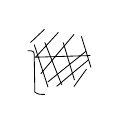
\begin{tikzpicture}[x={\dimexpr\dimen0/578\relax},y={\dimexpr-\dimen2/326\relax},line width=.3pt]
\path[use as bounding box] (0,0) rectangle (578,326);
\draw (0,109)..controls (45,108) and (55,112)..(55,130)--(60,305)..controls (85,316) and (116,318)..(144,316);
\draw (24,70)--(141,8) (68,139)--(258,22) (110,218)--(389,32) (169,257)--(491,111) (243,278)--(513,151) (388,279)--(494,196);
\draw (55,80)--(171,282) (144,70)--(285,270) (298,70)--(393,248) (451,41)--(531,188);
\draw (56,140)--(526,132);
\end{tikzpicture}}}%
\kern4pt\box0\kern4pt\endgroup}

b) Une biextension de ${}_nP\times Q$ par $G$, i.e. un accouplement
\diagram{\begin{tikzcd}[ampersand replacement=\&]{}_nP\times{}_nQ\arrow[r,"\varphi"]\&G\end{tikzcd}}

\deleted{Avec \unsure{le|la|les}} Ces deux $(E',\varphi)$ satisfont la condition que
\[\varphi|({}_nP'\times{}_nQ)=E'(n)\]

\margin{\figure{\begin{tikzpicture}\fill (0,.45) circle (.02);\fill (0,0) circle (.03);\end{tikzpicture}}}
Un hom de biextensions $E_1\longrightarrow E_2$ définit un hom $(E'_1,\varphi_1)\mathbin{-}(E'_2,\varphi_2)$, \begingroup
\setbox0=\hbox{i.e. \inserted{(déf)} un hom de}
\dimen0=\wd0 \advance\dimen0 by 8pt
\dimen2=\ht0 \advance\dimen2 by \dp0 \advance\dimen2 by 8pt
\leavevmode\rlap{\raisebox{\dimexpr-\dp0-4pt\relax}{%
\begin{tikzpicture}[x={\dimexpr\dimen0/365\relax},y={\dimexpr-\dimen2/92\relax},line width=.3pt]
\path[use as bounding box] (0,0) rectangle (365,92);
\draw (117,68)..controls (126,38) and (182,43)..(203,21);
\end{tikzpicture}}}%
\kern4pt\box0\kern4pt\endgroup biextensions $u:E'_1\unsure{\longrightarrow|\mathbin{-}}E'_2$\raisebox{-1ex}{\begin{tikzpicture}[x=.04cm,y=.04cm]\draw (0,0)..controls (-.12,-.4) and (-.1,-.8)..(0,-1);\end{tikzpicture}}, tel que $\varphi\sim$

\uline{Je dis que le foncteur} $E\longmapsto(E',\varphi)$ \uline{est une équiv. de catégories}.

\begingroup
\setbox0=\hbox{%
  \let\ScanOverlaySavedSout\sout
  \let\sout\relax
  \deleted{%
    \let\sout\ScanOverlaySavedSout
    \parbox{.95\linewidth}{\deleted{a) \uline{\unsure{pl. fid.}}}\quad\deleted{b) \unsure{pl. fid.|pl fd}}
\[
\deleted{\text{i.e.}\quad\text{a)}\quad\operatorname{Hom}(P\otimes Q,\unsure{G|C})\xrightarrow{\sim}\operatorname{Hom}(P'\otimes Q,G)}
\]
\[\deleted{\text{b)}\quad E_1\simeq E_2\quad\text{ssi}\quad(E'_1,\varphi_1)\simeq(E'_2,\varphi_{\unsure{2|1}})}\]
\uline{Pl. fidèle} signifie aussi que $E\vdash E|(P',Q)$ est pl. fd, \unsure{i.e.|ou} encore, \deleted{\unsure{que|par}} par la suite exacte, \unsure{que|pour}
\[
\unsure{\text{et}|(*)}\quad\operatorname{Hom}(P''\otimes Q,\unsure{G|C})=0,\qquad
\inserted{(**)}\quad\operatorname{Hom}(P\otimes Q,\unsure{G|C})\longrightarrow\operatorname{Hom}(P'\otimes Q,\unsure{G|C})\quad\uuline{\text{surj.}}
\]
\deleted{\unsure{Ce qui est} \illegible{1} \unsure{ainsi}}
\deleted{\inserted{$(***)$} si $\unsure{E_1,E_2}$ tel que $\unsure{(E'_1,\varphi_1)|(E',\varphi)}$ $\unsure{\simeq}\ \unsure{1}$ \unsure{alors} $\unsure{E_1\simeq E_2|E_1\sim E_2}$}
\inserted{Si $E$ est tel que $E'\simeq1$, $\varphi=0$, alors $E\simeq1$}

La première assertion résulte de a) et b) qui impliquent $P''\otimes Q=0$, la deuxième résulte de c) [dans la deuxième alternative de c) les deux mbs de $(**)$ sont nuls!]:

\deleted{\uline{\unsure{Ess. surj}}.} \unsure{Pour|Par} $(***)$, on note que si $E'=0$, Alors par la suite ex.\unsure{te|de} $E$ est déterminé par un élément de $\operatorname{Ext}(P''\otimes^{\unsure{L}}Q,\unsure{G|C})$, \unsure{or|à} ceci équivaut : un élément de $\operatorname{Hom}(P''\otimes_{\unsure{-|1}}Q,G)$, on \unsure{donne|trouve} que c'est ce qui définit \unsure{$\varphi$, on|$\varphi_1=0$} gagne.}}}
\dimen0=\wd0 \advance\dimen0 by 8pt
\dimen2=\ht0 \advance\dimen2 by \dp0 \advance\dimen2 by 8pt
\leavevmode\rlap{\raisebox{\dimexpr-\dp0-4pt\relax}{%
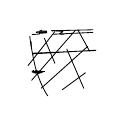
\begin{tikzpicture}[x={\dimexpr\dimen0/1476\relax},y={\dimexpr-\dimen2/1080\relax},line width=.3pt]
\path[use as bounding box] (0,0) rectangle (1476,1080);
\draw (6,597)--(584,60) (83,827)--(1029,36) (288,951)--(1289,292) (736,976)--(1240,706);
\draw (45,131)..controls (58,254) and (150,596)..(177,651)..controls (237,805) and (357,1001)..(432,1071);
\draw (72,215)--(78,289)--(65,263);
\draw (357,163)--(584,561) (1075,34)--(1330,373) (836,332)--(1204,954);
\draw (94,412)--(1465,353) (94,401)--(1465,358);
\draw (548,48)--(1402,33) (546,103)--(1404,74);
\draw (176,67)--(410,62) (176,74)--(410,68) (238,90)--(415,80);
\draw (262,51)..controls (279,35) and (309,39)..(291,51)--(248,55)--(403,54)..controls (411,57) and (414,62)..(408,70);
\draw (89,109)--(266,98);
\draw (531,58)..controls (504,46) and (520,37)..(540,45)--(748,59)..controls (781,62) and (700,78)..(688,91)..controls (670,104) and (725,109)..(785,104);
\draw (91,697)--(367,686);
\draw (90,688)--(123,673)--(119,699)--(162,679)--(147,705)--(197,681)--(180,709)--(231,685)--(212,712)--(259,690)--(244,714)--(290,689)--(279,708)--(329,694);
\end{tikzpicture}}}%
\kern4pt\box0\kern4pt\endgroup

\uline{Corollaire} 1 Supposons, pour un \begingroup
\setbox0=\hbox{$\mathbb{P}$ de \unsure{nbs|nb} premiers}
\dimen0=\wd0 \advance\dimen0 by 8pt
\dimen2=\ht0 \advance\dimen2 by \dp0 \advance\dimen2 by 8pt
\leavevmode\rlap{\raisebox{\dimexpr-\dp0-4pt\relax}{%
\begin{tikzpicture}[x={\dimexpr\dimen0/665\relax},y={\dimexpr-\dimen2/65\relax},line width=.3pt]
\path[use as bounding box] (0,0) rectangle (665,65);
\draw (179,9)--(215,52);
\end{tikzpicture}}}%
\kern4pt\box0\kern4pt\endgroup que
\[\left(\varinjlim_{\substack{n\\\text{\unsure{composé|à support}}\ \mathbb{P}}}{}_nP\right)\longrightarrow P''\quad\text{surjectif},\qquad\text{et que}\quad p\in\mathbb{P}\Longrightarrow pQ=Q.\]
Alors on a une équivalence $E\vdash(E',\varphi)$, \unsure{i.e.|où} $E$ est \unsure{une|un}
\margin{47}

\scanpage{49}
\margin{15}
topologiques paracompacts, à un théorème d'isomorphisme pour les \deleted{préfa} préfaisceaux [T.F Chap. II, § 5, Th. 10.2] comme on s'en convaint facilement en examinant le cas des préfaisceaux constants.

Cependant, la notion introduite ici coincide avec celle de [T.F.] dans le cas particulier des préfaisceau abéliens $P$ tel que $P(\varnothing)=0$, condition vérifiée par exemple par les préfaisceaux $\mathcal H^q(F)$ \deleted{\unsure{fa|qui}} qui s'introduisent dans la suite spectrale de Leray.
\margin{\begingroup
\setbox0=\hbox{\rotatebox{18}{aligner}}
\dimen0=\wd0 \advance\dimen0 by 8pt
\dimen2=\ht0 \advance\dimen2 by \dp0 \advance\dimen2 by 8pt
\leavevmode\rlap{\raisebox{\dimexpr-\dp0-4pt\relax}{%
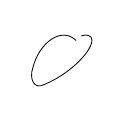
\begin{tikzpicture}[x={\dimexpr\dimen0/229\relax},y={\dimexpr-\dimen2/140\relax},line width=.3pt]
\path[use as bounding box] (0,0) rectangle (229,140);
\draw (161,26) .. controls (113,-3) and (38,30) .. (17,82) .. controls (5,103) and (20,128) .. (57,115) .. controls (130,97) and (210,53) .. (214,26) .. controls (215,16) and (194,12) .. (178,17);
\end{tikzpicture}}}%
\kern4pt\box0\kern4pt\endgroup
\figure{\begin{tikzpicture}[x=1cm,y=1cm]\draw (2.7,2.17)--(2.2,2.1);\draw (2.31,2.27)--(2.2,2.1)--(2.29,1.98);\draw (2.16,1.86)--(2.16,.34);\draw (1.92,1.52)--(2.03,1.65);\draw (2.52,0)--(2.09,.2);\draw (2.3,.27)--(2.09,.2)--(2.22,.09);\end{tikzpicture}}}

Enfin soit $\deleted{\unsure{A|\lambda}}\ a:\widehat C_A\longrightarrow\widetilde C_A$ le foncteur faisceau associé. Le foncteur $a$ est exact. Il est adjoint à gauche au foncteur $\mathcal H^0$. Le morphisme d'adjonction :
\[a\mathcal H^0\longrightarrow\operatorname{id}_{\widetilde C_A}\qquad(21)\]
est un isomorphisme (2.3.14.II).

La formule d'adjonction fournit pour tout préfaisceau d'ensembles $S$ sur $C$ et tout faisceau \begingroup
\setbox0=\hbox{d\raisebox{.65ex}{\inserted{\unsure{e|'}}}e}
\dimen0=\wd0 \advance\dimen0 by 8pt
\dimen2=\ht0 \advance\dimen2 by \dp0 \advance\dimen2 by 8pt
\leavevmode\rlap{\raisebox{\dimexpr-\dp0-4pt\relax}{%
\begin{tikzpicture}[x={\dimexpr\dimen0/73\relax},y={\dimexpr-\dimen2/54\relax},line width=.3pt]
\path[use as bounding box] (0,0) rectangle (73,54);
\draw (24,39) .. controls (33,39) and (43,36) .. (51,30);
\end{tikzpicture}}}%
\kern4pt\box0\kern4pt\endgroup $A$-modules $F$ un isomorphisme :
\margin{$\unsure{\rho}$ \raisebox{-.7ex}{\begin{tikzpicture}[x=.06cm,y=-.06cm]\draw[line width=.7pt] (0,0)--(1,.5);\end{tikzpicture}}}
\inserted{$F(aS)\xrightarrow{\sim}\mathcal H^0(F)(\unsure{S|s})$ i.e.:}
\margin{$\unsure{\rho}$}
\[
\deleted{H^0(C/aS,F)\ \unsure{\longrightarrow}\ H^0(\unsure{\widehat C|C}/S,F)\unsure{=|-}H^0(\widehat C/S,}
\]
\[H^0(\widetilde C/aS,F)\xrightarrow{\sim}H^0(\widehat C/S,\mathcal H^0(F))\qquad(22)\]

De plus si $G$ est un préfaisceau de $A$-modules tel que le faisceau associé soit nul, on a ((2.3.12.II) et (2.3.14.II)) :
\[\check{\mathcal H}^{0}(G)=0\qquad(23)\]
\margin{\begingroup
\setbox0=\hbox{\shortstack[l]{Laisser ici\\un interligne}\hspace{2.5cm}}
\dimen0=\wd0 \advance\dimen0 by 8pt
\dimen2=\ht0 \advance\dimen2 by \dp0 \advance\dimen2 by 8pt
\leavevmode\rlap{\raisebox{\dimexpr-\dp0-4pt\relax}{%
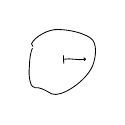
\begin{tikzpicture}[x={\dimexpr\dimen0/575\relax},y={\dimexpr-\dimen2/260\relax},line width=.3pt]
\path[use as bounding box] (0,0) rectangle (575,260);
\draw (44,71)--(32,61) .. controls (56,35) and (175,4) .. (257,7) .. controls (385,8) and (544,30) .. (556,58) .. controls (583,90) and (553,142) .. (522,161) .. controls (456,210) and (277,264) .. (201,250) .. controls (142,235) and (99,224) .. (64,227) .. controls (43,224) and (32,220) .. (29,215) .. controls (8,193) and (10,161) .. (15,144) .. controls (16,112) and (27,89) .. (40,77);

\draw (299,105)--(301,136);
\draw (306,119) .. controls (361,114) and (420,125) .. (483,119);
\draw (468,113)--(483,119)--(471,125);
\end{tikzpicture}}}%
\kern4pt\box0\kern4pt\endgroup}

Nous allons maintenant én\deleted{n}oncer les propositions liant la cohomologie de \leavevmode\rlap{\raisebox{.85ex}{\inserted{\v{\phantom{C}}}}}Cech à la cohomologie des faisceaux.

\uline{Proposition 2.2} : Le foncteur $\mathcal H^0$ transforme les faisceaux injectifs en préfaisceaux injectifs. Soit $F$ un faisceau de $A$-modules. Les faisceaux associés aux préfaisceaux $\mathcal H^q(F)$ $(q>0)$ sont nuls.
\margin{\figure{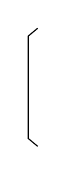
\begin{tikzpicture}\draw (.12,1.5)--(0,1.4)--(0,.1)--(.12,0);\end{tikzpicture}}}

\uline{Preuve} : Le foncteur faisceau associé, adjoint à gauche du foncteur $\mathcal H^0$ est exact; d'où la première assertion (0.2). Le foncteur $a\mathcal H^0$ est isomorphe au foncteur identique (formule (21)) d'où la deuxième assertion.

\uline{Proposition 2.3} : Soit $S$ un préfaisceau d'ensembles sur $C$.

Il existe une suite spectrale fonctoriel\raisebox{.45ex}{\inserted{le}} en $S$ et $F$ :
\[\deleted{H^{p+q}(C/\unsure{X|Y},F)\qquad\unsure{H}}\]
\[\vcenter{\hbox{\begingroup
\setbox0=\hbox{$\displaystyle H^{p+q}(\widetilde C/aS,F)\Longleftarrow H^p(\widehat C/S,\mathcal H^q(\unsure{\deleted{E}F|\deleted{F}E}))$}
\dimen0=\wd0 \advance\dimen0 by 18pt
\dimen2=\ht0 \advance\dimen2 by \dp0 \advance\dimen2 by 16pt
\rlap{\raisebox{\dimexpr-\dp0-8pt\relax}{%
\begin{tikzpicture}[x={\dimexpr\dimen0/647\relax},y={\dimexpr-\dimen2/74\relax},line width=.3pt]
\path[use as bounding box] (0,0) rectangle (647,74);
\draw (400,-18)..controls (401,-7) and (402,5)..(403,14);\draw (403,17)--(403,24);\draw (403,27)--(403,31);
\end{tikzpicture}}}%
\kern9pt\box0\kern9pt\endgroup}}\]
\margin{\figure{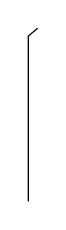
\begin{tikzpicture}\draw (.12,2.2)--(0,2.1)--(0,0);\end{tikzpicture}}}
\margin{48}

\scanpage{50}
biextension \deleted{\unsure{de}} de $P,Q$ par $G$, et où $(E',\varphi)$ est le couple d'une biext. $E'$ de $P',Q$ par $G$ et d'un hom
\diagram{\begin{tikzcd}[ampersand replacement=\&]\varphi:T_{\mathbb P}(P)\times T_{\mathbb P}(Q)\arrow[r]\&T_{\mathbb P}(G)\end{tikzcd}}
\uline{qui étend l'hom}
\diagram{\begin{tikzcd}[ampersand replacement=\&]\deleted{\unsure{\varphi}}\ \varphi_{\mathbb P,E'}:T_{\mathbb P}(P')\times T_{\mathbb P}(Q)\arrow[r,no head]\&T_{\mathbb P}(G)\end{tikzcd}}

\margin{\begingroup
\setbox0=\hbox{\parbox{.65\linewidth}{$2$\quad\uline{NB} On considère les $T_{\mathbb P}(P)$ comme syst. projectifs \deleted{\uline{par suite}} \deleted{\uline{\unsure{stricts}}}, \unsure{\deleted{elle est vraie}|\inserted{elle est vraie}}\\cette description \unsure{ne marche que} \deleted{(\unsure{en|un} \unsure{termes|hom} de syst. projectifs \unsure{sans passage à la limite})}\\si $\forall p\in\mathbb P$ \unsure{on a|: --}\\ -- $pP'\unsure{=|\cdot}P'$, $pP''=pP''$ donc $pP=pP$. Sinon,\\ il faut garder le syst. des ${}_nP\times{}_nQ\mathbin{-}{}_nG$\\ \deleted{\unsure{prolongeant} ${}_mP'\times{}_mQ'\unsure{\longrightarrow|\mathbin{-}}{}_mG$} avec la compatibilité\\ pour $n$ et $m$ \uline{et} la compatibilité de restriction aux ${}_{\unsure{n|m}}P'\times{}_nQ\ \ldotp\ldotp\ldotp\ldotp\ldotp$}}
\dimen0=\wd0 \advance\dimen0 by 8pt
\dimen2=\ht0 \advance\dimen2 by \dp0 \advance\dimen2 by 8pt
\leavevmode\rlap{\raisebox{\dimexpr-\dp0-4pt\relax}{%
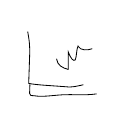
\begin{tikzpicture}[x={\dimexpr\dimen0/680\relax},y={\dimexpr-\dimen2/445\relax},line width=.3pt]
\path[use as bounding box] (0,0) rectangle (680,445);
\draw (0,25) .. controls (18,88) and (22,126) .. (20,170) -- (10,360) .. controls (80,370) and (220,374) .. (359,381) .. controls (433,390) and (502,375) .. (550,369);
\draw (22,367) -- (19,425) .. controls (17,443) and (38,437) .. (64,440) .. controls (145,449) and (237,438) .. (340,434) .. controls (463,430) and (561,439) .. (680,428);
\draw (285,201) .. controls (294,244) and (342,260) .. (402,270);
\draw (400,270) -- (401,157) .. controls (430,206) and (452,217) .. (469,209) .. controls (483,195) and (482,135) .. (497,119) .. controls (522,151) and (595,146) .. (638,136);
\end{tikzpicture}}}%
\kern4pt\box0\kern4pt\endgroup}

\uline{Corollaire} 1 Soient deux suites exactes
\diagram{\begin{tikzcd}[ampersand replacement=\&, column sep=small]
\cdot\arrow[r,no head]\&P'\arrow[r,no head]\&P\arrow[r,no head]\&P''\arrow[r,no head]\&\unsure{\cdot|0}\\
\cdot\arrow[r,no head]\&Q'\arrow[r,no head]\&Q\arrow[r]\&Q''\arrow[r]\&0
\end{tikzcd}}
et supposons que, pour un $\mathbb P$ de nbs premiers, on ait :
\[\unsure{\text{a}|\cdot})\quad p\in\mathbb P\Longrightarrow p\underline{P=P},\quad p\underline{Q'=Q'}\quad
\deleted{et\ pQ''=Q''\ \unsure{ou}\ \unsure{p\underline{P''=pP''}|p\underline{P''=P''}}}
\]
\inserted{(ou le symétrique)}
\margin{\begingroup
\setbox0=\hbox{\shortstack[l]{\deleted{(\unsure{donc} $pP=P$, $pQ=\unsure{0|Q}$)}\\[3ex]\strut}}
\dimen0=\wd0 \advance\dimen0 by 8pt
\dimen2=\ht0 \advance\dimen2 by \dp0 \advance\dimen2 by 8pt
\leavevmode\rlap{\raisebox{\dimexpr-\dp0-4pt\relax}{%
\begin{tikzpicture}[x={\dimexpr\dimen0/340\relax},y={\dimexpr-\dimen2/125\relax},line width=.3pt]
\path[use as bounding box] (0,0) rectangle (340,125);
\draw (-3,47)..controls (28,65) and (118,56)..(151,91)..controls (178,125) and (137,126)..(156,109)..controls (192,82) and (257,86)..(288,73);
\end{tikzpicture}}}%
\kern4pt\box0\kern4pt\endgroup}
\[
\text{b)}\quad\text{les.}\quad\varinjlim_{n\to\mathbb P}{}_nP\longrightarrow P''\quad\text{et}\quad
\underset{n\to\mathbb P}{\underline{\lim}}{}_nQ\mathbin{-}Q''\quad\text{épim.}
\]
\figure{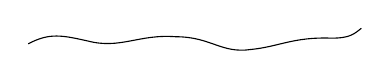
\begin{tikzpicture}[x=.018cm,y=-.018cm]
\draw (9,36) .. controls (24,28) and (33,30) .. (51,34) .. controls (74,40) and (87,29) .. (113,31) .. controls (138,31) and (145,43) .. (166,40) .. controls (186,38) and (196,31) .. (223,32) .. controls (236,32) and (239,29) .. (244,25);
\end{tikzpicture}}
\margin{\begingroup
\setbox0=\hbox{\parbox{.65\linewidth}{\unsure{Ne vaut que}, \unsure{celle en modules|cela ne marche} tel quel que si on suppose que $P',Q;P'',\unsure{G'|Q'|G.}$\\ \unsure{sont} $\mathbb P$ divisibles dans a), en plus de b).\\ Sinon, garder les ${}_nP\times{}_nQ\longrightarrow{}_nG\ \ldotp\ldotp\ldotp\ldotp\ldotp$}}
\dimen0=\wd0 \advance\dimen0 by 8pt
\dimen2=\ht0 \advance\dimen2 by \dp0 \advance\dimen2 by 8pt
\leavevmode\rlap{\raisebox{\dimexpr-\dp0-4pt\relax}{%
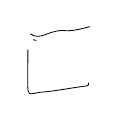
\begin{tikzpicture}[x={\dimexpr\dimen0/760\relax},y={\dimexpr-\dimen2/200\relax},line width=.3pt]
\path[use as bounding box] (0,0) rectangle (760,200);
\draw (30,18) .. controls (145,38) and (207,10) .. (382,8) .. controls (479,11) and (556,6) .. (686,-3);
\draw (2,64) .. controls (4,108) and (-5,166) .. (5,183) .. controls (13,199) and (69,190) .. (127,188) .. controls (318,184) and (495,174) .. (655,169) .. controls (670,169) and (674,166) .. (671,160);
\draw (59,35)--(96,37);
\end{tikzpicture}}}%
\kern4pt\box0\kern4pt\endgroup}

Alors le foncteur
\diagram{\begin{tikzcd}[ampersand replacement=\&]E\arrow[r,mapsto]\&(E',\varphi)\end{tikzcd}}
\unsure{associant à|associe à|envoyant} : \unsure{la|les} biext. de $P,Q$ par $G$ la restriction $E':P',Q'$ et la forme $\varphi_{E,\mathbb P}$
\diagram{\begin{tikzcd}[ampersand replacement=\&]\varphi:T_{\mathbb P}(P)\times T_{\mathbb P}(Q)\arrow[r,no head]\&T_{\mathbb P}(G)\end{tikzcd}}
prolongeant
\diagram{\begin{tikzcd}[ampersand replacement=\&]\varphi_{E',\mathbb P}:T_{\mathbb P}(P')\times T_{\mathbb P}(Q')\arrow[r,no head]\&T_{\mathbb P}(G)\end{tikzcd}}
est une équivalence de catégories.

\uline{Dém.} \inserted{\unsure{Supposons} p.ex.} On applique d'abord \begingroup
\setbox0=\hbox{\shortstack[l]{\hspace{1em}\deleted{\unsure{proposition}}\\le\quad corollaire 1 à}}
\dimen0=\wd0 \advance\dimen0 by 8pt
\dimen2=\ht0 \advance\dimen2 by \dp0 \advance\dimen2 by 8pt
\leavevmode\rlap{\raisebox{\dimexpr-\dp0-4pt\relax}{%
\begin{tikzpicture}[x={\dimexpr\dimen0/530\relax},y={\dimexpr-\dimen2/190\relax},line width=.3pt]
\path[use as bounding box] (0,0) rectangle (530,190);
\draw (98,136)..controls (80,110) and (120,86)..(166,86)..controls (230,82) and (291,75)..(294,68);
\end{tikzpicture}}}%
\kern4pt\box0\kern4pt\endgroup
\diagram{\begin{tikzcd}[ampersand replacement=\&, column sep=small]0\arrow[r,no head]\&P'\arrow[r]\&P\arrow[r,no head]\&P''\arrow[r,no head]\&\unsure{\cdot|0}\end{tikzcd}}
et $Q'$, en utilisant $pQ'=Q'$, $\underset{\unsure{\longrightarrow|\mathbin{-}}}{\lim}{}_nP\longrightarrow P''$ épim.

Cela donne une description des biextensions de $P,Q'$. On applique ensuite le sym. du cor. 1 à $P$ et
\diagram{\begin{tikzcd}[ampersand replacement=\&, column sep=small]\unsure{\cdot|0}\arrow[r]\&Q'\arrow[r]\&Q\arrow[r]\&Q''\arrow[r]\&0,\end{tikzcd}}
en utilisant $pP=P$ \begingroup
\setbox0=\hbox{\deleted{\unsure{i.e.|et} $\unsure{pP''=P''}$}}
\dimen0=\wd0 \advance\dimen0 by 8pt
\dimen2=\ht0 \advance\dimen2 by \dp0 \advance\dimen2 by 8pt
\leavevmode\rlap{\raisebox{\dimexpr-\dp0-4pt\relax}{%
\begin{tikzpicture}[x={\dimexpr\dimen0/270\relax},y={\dimexpr-\dimen2/125\relax},line width=.3pt]
\path[use as bounding box] (0,0) rectangle (270,125);
\draw (61,58) -- (60,48) .. controls (102,61) and (142,42) .. (216,43) -- (217,38);
\end{tikzpicture}}}%
\kern4pt\box0\kern4pt\endgroup et $\varinjlim_{n\to\mathbb P}{}_nQ\mathbin{-}Q''$ épim.
\margin{49}

\scanpage{51}
\mspage{13}
\[
\mathcal H^0:\widetilde C_A\longrightarrow\widehat C_A \qquad(10)
\]
le foncteur d'injection des faisceaux dans les préfaisceaux.
Le foncteur $\mathcal H^0$ est un foncteur exact à gauche (2.3.14.II).
Ses foncteurs dérivés \unsure{droitsseront|droits seront} notés :
\[
\mathcal H^q:\widetilde C_A\longrightarrow\widehat C_A \qquad(11)
\]
Pour tout objet $X$ de $C$ \deleted{,\unsure{on a}} et pour tout A-Module $F$, on a :
\[
\inserted{\mathcal H^q(F)(X)}\;\deleted{\unsure{t|\dagger}\,\unsure{\mathcal H^q|H^q}}\;
\deleted{H^0(\unsure{\widehat C}/X,\mathcal H^q(F))}=H^q(\widetilde C/X,F)\qquad(12)
\]
En effet pour $q=0$, cet isomorphisme résulte immédiatement des définitions. On l'en déduit pour tout $q$ en remarquant que le foncteur ``section\inserted{s} sur $X$'' est exact \deleted{\unsure{à|d}} sur la catégorie des préfaiscea\deleted{\illegible{2}}\unsure{ux}.

Soit $L:\widehat C\longrightarrow\widehat C$ le foncteur défini en (2.3.11.II).
Le foncteur $L$ commute aux limites projectives finies et par suite transforme \margin{\raisebox{.7ex}{$\unsure{\rho}$}\,\inserted{les}} $\unsure{\rho}$ préfaisceaux d' A-modules en préfaisceaux de A-modules. Nous noterons :
\[
\check{\mathcal H}^{0}:\widehat C_A\longrightarrow\widehat C_A \qquad(13)
\]
\margin{\figure{\begin{tikzpicture}[x=1mm,y=1mm]
\draw[line width=0.3pt,black!30] (0,46.9) -- (9,46.5);
\draw[line width=0.25pt,black!20] (9,46.5) -- (9,0.2);
\draw[line width=0.3pt,black!45] (9,44.8) -- (9,43.2) (9,42.7) -- (9,41.9);
\draw[line width=0.5pt,black!75] (0,0.6) .. controls (3,0.25) and (6,0.05) .. (9,0.2);
\end{tikzpicture}}}
\margin{\figure{\begin{tikzpicture}[x=1mm,y=1mm]
\draw[line width=0.5pt,black!40] (0,0) -- (1.8,2.2);
\draw[line width=0.7pt] (1.3,1.6) -- (1.8,2.2);
\end{tikzpicture}}}
le foncteur induit par $L$ sur les préfaisceaux de A-modules.
Le foncteur $\check{\mathcal H}^0$ est exact à \deleted{droite} gauche. Ses foncteurs dérivés droits seront notés $\check{\mathcal H}^q$. \deleted{Les préfai} Soit $G$ un préfaisceau de A-modules. Les préfaisceaux $\check{\mathcal H}^q(G)$ seront appelés les préfaisceaux de \begingroup
\setbox0=\hbox{cohomologie de \v{C}ech du}
\dimen0=\wd0 \advance\dimen0 by 8pt
\dimen2=\ht0 \advance\dimen2 by \dp0 \advance\dimen2 by 8pt
\leavevmode\rlap{\raisebox{\dimexpr-\dp0-4pt\relax}{%
\begin{tikzpicture}[x={\dimexpr\dimen0/390\relax},y={\dimexpr-\dimen2/80\relax},line width=.3pt]
\path[use as bounding box] (0,0) rectangle (390,80);
\draw (22,65) .. controls (130,66) and (261,68) .. (365,69);
\end{tikzpicture}}}%
\kern4pt\box0\kern4pt\endgroup préfaisceau $G$.

Ppour tout objet $X$ de $C$, on a un isomorphisme canonique :
\begingroup
\setbox0=\hbox{%
  \let\ScanOverlaySavedSout\sout
  \let\sout\relax
  \deleted{%
    \let\sout\ScanOverlaySavedSout
    \parbox{.95\linewidth}{\[\deleted{\unsure{H^0(\widehat C, H^0(\widehat C/X,\qquad(G)))=\operatorname{Lim}}}\]\[H^0(\widehat C/X,\qquad(G))=\underset R{\operatorname{Lim}}\,H^q(\widehat C/R,G)^{C}\]En effet pour $q=0$, cet isomorphisme résulte immédiatement\\des définitions}}}
\dimen0=\wd0 \advance\dimen0 by 8pt
\dimen2=\ht0 \advance\dimen2 by \dp0 \advance\dimen2 by 8pt
\leavevmode\rlap{\raisebox{\dimexpr-\dp0-4pt\relax}{%
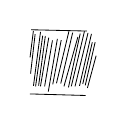
\begin{tikzpicture}[x={\dimexpr\dimen0/1045\relax},y={\dimexpr-\dimen2/265\relax},line width=.3pt]
\path[use as bounding box] (0,0) rectangle (1045,265);
\draw (51,8) -- (900,13);
\draw (35,255) -- (880,261);
\draw (36,114) -- (87,12);
\draw (44,177) -- (113,25);
\draw (88,224) -- (195,16);
\draw (120,226) -- (228,31);
\draw (166,223) -- (268,32);
\draw (194,226) -- (320,38);
\draw (257,226) -- (376,49);
\draw (313,246) -- (451,43);
\draw (381,218) -- (509,48);
\draw (437,214) -- (626,14);
\draw (502,215) -- (683,19);
\draw (551,226) -- (762,36);
\draw (619,230) -- (797,23);
\draw (662,226) -- (862,14);
\draw (719,226) -- (916,20);
\draw (787,224) -- (968,24);
\draw (836,217) -- (981,56);
\draw (874,222) -- (1024,56);
\draw (907,232) -- (1039,108);
\end{tikzpicture}}}%
\kern4pt\box0\kern4pt\endgroup
\[
\inserted{\check{\mathcal H}^q(G)(X)}\;\deleted{H^0(\unsure{\widehat C}/X,\check{\mathcal H}^q(G))}
=\vcenter{\hbox{\begingroup
\setbox0=\hbox{$\displaystyle \underset{R}{\underset{\longrightarrow}{\operatorname{Lim}}}$}
\dimen0=\wd0 \advance\dimen0 by 18pt
\dimen2=\ht0 \advance\dimen2 by \dp0 \advance\dimen2 by 16pt
\rlap{\raisebox{\dimexpr-\dp0-8pt\relax}{%
\begin{tikzpicture}[x={\dimexpr\dimen0/64\relax},y={\dimexpr-\dimen2/70\relax},line width=.3pt]
\path[use as bounding box] (0,0) rectangle (64,70);
\draw (2,31)--(14,3);
\end{tikzpicture}}}%
\kern9pt\box0\kern9pt\endgroup}}\,H^q(\widehat C/R,G)\qquad(14)
\]
\shortstack[l]{\inserted{Comme}\\\deleted{Ainsi qu'}} il resulte immédiatement des définitions (2.3.11.II).

(Dans cette formule la limite inductive est prise suivant la catégorie des cribles couvrants $X$).
\margin{50}

\scanpage{52}
\uline{Biextensions \unsure{sous hyp. de|sans hyp. de} rigidité}

$A,G$ faisceaux abéliens sur topos $\unsure{S|\mathcal S}$,
\begin{center}
\begin{tabular}{@{}l@{}l@{}}
$f:A\longrightarrow S$ &
\begin{tikzpicture}[overlay,baseline=0pt,x=1em,y=1ex]
\draw (-.2,.5) .. controls (.4,-.7) and (1.3,-2.2) .. (1.8,-2.5);
\end{tikzpicture}\\
& \hspace{1.6em}objet final
\end{tabular}
\end{center}

a) Supposons $\underline{\operatorname{Hom}}_{\unsure{grs|gr|gts|gtes}}(A,G)\simeq0$. Alors
\[
\operatorname{Ext}^1(A,G)\xrightarrow{\sim}H^0(S,\underline{\operatorname{Ext}}(A,G))
\]
donc la connaissance du \uline{faisceau} $\underline{\operatorname{Ext}}(A,G)$ implique celle de $\operatorname{Ext}(A,G)$ et ts des $\operatorname{Ext}(A_{\unsure{\bar s|T|\bar S}},G_{\unsure{\bar s|T|\bar S}})$.

b) Supposons $\underline{\operatorname{Hom}}_{pct}(A,G)=0$, Alors
\margin{\begingroup
\setbox0=\hbox{i.e. $f_{\unsure{*|\alpha}}(G_A)\xleftarrow{\sim}G$}
\dimen0=\wd0 \advance\dimen0 by 8pt
\dimen2=\ht0 \advance\dimen2 by \dp0 \advance\dimen2 by 8pt
\leavevmode\rlap{\raisebox{\dimexpr-\dp0-4pt\relax}{%
\begin{tikzpicture}[x={\dimexpr\dimen0/490\relax},y={\dimexpr-\dimen2/80\relax},line width=.3pt]
\path[use as bounding box] (0,0) rectangle (490,80);
\draw (28,75) .. controls (26,67) and (38,70) .. (65,69) -- (453,68) .. controls (475,70) and (478,62) .. (476,56);
\end{tikzpicture}}}%
\kern4pt\box0\kern4pt\endgroup}
\margin{\figure{\begin{tikzpicture}\draw(0,0)--(0,-.35);\end{tikzpicture}} Hom (pas \unsure{néc\textsuperscript{t}} multiplicatifs)\\qui respectent la section\\\unsure{unités|unité}}
\begin{center}
\begin{tabular}{@{}r@{\quad}l@{}}
$H^1(A,A_G)\simeq H^1(S,G)\times$ & $\vcenter{\hbox{\begingroup
\setbox0=\hbox{$\displaystyle H^0(S,R^1f_{\unsure{*|\alpha}}(G_A)$}
\dimen0=\wd0 \advance\dimen0 by 18pt
\dimen2=\ht0 \advance\dimen2 by \dp0 \advance\dimen2 by 16pt
\rlap{\raisebox{\dimexpr-\dp0-8pt\relax}{%
\begin{tikzpicture}[x={\dimexpr\dimen0/390\relax},y={\dimexpr-\dimen2/105\relax},line width=.3pt]
\path[use as bounding box] (0,0) rectangle (390,105);
\draw (30,78) .. controls (140,83) and (300,82) .. (365,80) .. controls (375,81) and (377,78) .. (372,73);
\end{tikzpicture}}}%
\kern9pt\box0\kern9pt\endgroup}}$\\
& \hspace{1em}\rotatebox{90}{$\simeq$}\\
& Classes \unsure{à|:} isom près de $G_A$-torseurs\\
& \deleted{\unsure{fou}} rigidi\uline{\unsure{fiés|fié}} rel. à $e_A$\\
& \hspace{1em}\rotatebox{90}{$\simeq$}\\
& Classes de \deleted{torseurs} $G_A$-torseurs\\
& rigidi\uline{fiables} rel. à $e_A$.\\
\end{tabular}
\end{center}
\margin{\figure{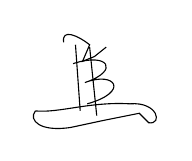
\begin{tikzpicture}[x=.03cm,y=-.03cm]
\draw (25,13) .. controls (24,7) and (31,10) .. (36,14) -- (33,21) -- (38,19) -- (43,15);
\draw (30,14) -- (32,42);
\draw (36,15) -- (39,44);
\draw (29,22) .. controls (44,17) and (49,25) .. (34,30) .. controls (47,25) and (53,34) .. (35,39);
\draw (13,42) .. controls (23,43) and (36,38) .. (53,39) .. controls (65,38) and (67,48) .. (61,47) -- (57,43) -- (42,46) -- (28,49) .. controls (15,51) and (10,46) .. (13,42);
\end{tikzpicture}}}

De plus, le foncteur oubli, qui va de la catégorie des extensions de $A$ par $G$ en \unsure{la} catégorie des $G_A$-torseurs $e_A$-rigidifiés, est un fonct pl. fid. (de catégories discrètes), (\deleted{\unsure{d'où|donc}}. on a une \uline{injection}
\[
0\longrightarrow\operatorname{Ext}^1(A,G)\longrightarrow H^1(A,G_A)
\]
); l'image essentielle est formée des \begingroup
\setbox0=\hbox{\begingroup\let\sout\relax\shortstack[l]{\hspace{2.6em}\deleted{\inserted{\unsure{fib}}}\\\deleted{\unsure{classes}\quad$G_A$}}\endgroup}
\dimen0=\wd0 \advance\dimen0 by 8pt
\dimen2=\ht0 \advance\dimen2 by \dp0 \advance\dimen2 by 8pt
\leavevmode\rlap{\raisebox{\dimexpr-\dp0-4pt\relax}{%
\begin{tikzpicture}[x={\dimexpr\dimen0/305\relax},y={\dimexpr-\dimen2/90\relax},line width=.3pt]
\path[use as bounding box] (0,0) rectangle (305,90);
\draw (110,36) -- (211,38);
\draw (14,60) -- (292,63);
\end{tikzpicture}}}%
\kern4pt\box0\kern4pt\endgroup-torseurs \begingroup
\setbox0=\hbox{\begingroup\let\sout\relax\shortstack[l]{\inserted{tels que}\\\deleted{\unsure{classes.|classe.}\ \unsure{rigi}\quad$\xi$\quad\unsure{telles|telle}}}\endgroup}
\dimen0=\wd0 \advance\dimen0 by 8pt
\dimen2=\ht0 \advance\dimen2 by \dp0 \advance\dimen2 by 8pt
\leavevmode\rlap{\raisebox{\dimexpr-\dp0-4pt\relax}{%
\begin{tikzpicture}[x={\dimexpr\dimen0/550\relax},y={\dimexpr-\dimen2/102\relax},line width=.3pt]
\path[use as bounding box] (0,0) rectangle (550,102);
\draw (12,80) -- (533,46);
\end{tikzpicture}}}%
\kern4pt\box0\kern4pt\endgroup
\[
\pi^{\unsure{*|\alpha}}(\deleted{\unsure{F|\xi}}L)\simeq\operatorname{pr}_1^{\unsure{*|\alpha}}(L)\operatorname{pr}_2(L)
\]
i.e tels que
\[
\pi^{\unsure{*|\alpha}}(L)\operatorname{pr}_1^{\unsure{*|\alpha}}(L)^{-1}\operatorname{pr}_2^{\unsure{*|\alpha}}(L)^{-1}\simeq0.
\]
On trouve encore comme corollaire une suite exacte
\margin{\diagram{\begin{tikzcd}[ampersand replacement=\&,column sep=large]
A\times A\arrow[r,shift left=2.5ex,"\operatorname{pr}_1"]\arrow[r,"\operatorname{pr}_2"]\arrow[r,shift right=2.5ex,"\pi"]\&A
\end{tikzcd}}}
\diagram{\begin{tikzcd}[ampersand replacement=\&,column sep=small,row sep=large]
\unsure{\bullet|0}\arrow[r,no head]\&\underline{\operatorname{Ext}}^1(A,G)\arrow[rr,"i"]\&\&R^1f_{\unsure{*|\alpha}}(G_A)\arrow[r,"j"]\arrow[dl,"k"']\&\underline{\operatorname{Tors}}\ \underline{\mathrm{birig}}\ \underline{\mathrm{sym}}(A,A;G)\\
\text{i.e.}\&\unsure{\bullet|0}\arrow[r,phantom,"\unsure{\mathbin{-}|\longrightarrow}" description]\&\underline{\mathrm{NS}}(A)\arrow[rr,"\deleted{\unsure{k}}","j'"']\&\&\underline{\operatorname{Tors}\ \mathrm{birig}}\ \underline{\mathrm{sym}}(\unsure{A|B},A;G)\arrow[u,phantom,shift left=8ex,"\unsure{\wr|i}" description]\arrow[u,phantom,shift left=3ex,"\text{''}" description]
\end{tikzcd}}
\margin{51}

\cotefile{36}
\scanpage{53}
\mspage{-1.6-}

$\phi:V_1\longrightarrow V_2$ commuting with the dual actions, then $\phi\circ E_1=E_2\circ\phi$ where $E_1$ and $E_2$ are the Reynolds operators on $V_{\unsure{1|i}}$ and $V_2$ respectively.

Suppose $V$ is actually a ring $R$, and $\hat\sigma$ is an action on the ring. Then the image of $E$ is\makebox[0pt][r]{\raisebox{-0.55em}[0pt][0pt]{\tikz[x=1em,y=1em]{\draw[line width=.3pt] (0,.04) .. controls (.08,-.02) and (.20,-.02) .. (.28,.05);}}\hspace{.03em}} the subspace of invariant elements of $R$, which is a \uline{subring} $R_0$ of $R$. Although $E$ is not a ring homomorphism, it satisfies the well-known Reynolds identity:
\[
(*)\qquad\text{If }x\in R,\ y\in R_0,\text{ then }E(x.y)=(Ex)\cdot y.
\]
(cf. Cartier\unsure{,} [6], 7-08). To prove this, set $R_1=\ker(E)$. Then $R\cong R_0\oplus R_1$, and $(*)$ is equivalent to the 2 statements $R_0\cdot R_0\subset R_0$ and $R_0\cdot R_1\subset R_1$. To prove the latter, let $g\in R_0$, and let $V\subset R_1$ be a (finite dimensional) irreducible invariant subspace. Then either $g\cdot V=(0)$ or multiplication by $g$ sets up an isomorphism of $V$ with an irreducible invariant subspace $g\cdot V$. Since $g$ is an invariant, the representations of $G$ on $V$ and $g\cdot V$ are isomorphic and non-trivial. Therefore $g\cdot V\subset R_1$.

\begingroup
\setbox0=\hbox{\S2.}
\dimen0=\wd0 \advance\dimen0 by 8pt
\dimen2=\ht0 \advance\dimen2 by \dp0 \advance\dimen2 by 8pt
\leavevmode\rlap{\raisebox{\dimexpr-\dp0-4pt\relax}{%
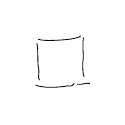
\begin{tikzpicture}[x={\dimexpr\dimen0/105\relax},y={\dimexpr-\dimen2/84\relax},line width=.3pt]
\path[use as bounding box] (0,0) rectangle (105,84);
\draw (16,14) .. controls (23,17) and (55,15) .. (65,14) .. controls (72,13) and (78,12) .. (81,10);
\draw (14,19) .. controls (17,29) and (14,42) .. (17,51) .. controls (18,55) and (15,61) .. (18,64);
\draw (85,12) .. controls (83,24) and (86,33) .. (84,43) .. controls (84,50) and (84,56) .. (86,60);
\draw (12,70) .. controls (23,74) and (48,73) .. (61,71) .. controls (67,72) and (70,70) .. (71,68);
\draw (75,69) .. controls (82,70) and (90,67) .. (95,68);
\end{tikzpicture}}}%
\kern4pt\box0\kern4pt\endgroup With these preliminaries disposed of, we can now take up the first case of the theory - the action of a reductive algebraic group on an affine scheme $X$. To keep straight the techniques in the proof, we do not assume that $X$ is an algebraic scheme over $k$.

\uline{Theorem} \uline{1.1}: Let $X$ be an affine scheme over $k$, let $G$ be a reductive algebraic group, and let $\sigma:G\mathbin{x}X\longrightarrow X$ be an action of $G$ on $X$. Then a universal categorical quotient $(Y,\phi)$ of $X$ by $G$

\margin{52}

\scanpage{54}

c) \deleted{\unsure{Soient|Soit}} $B$ un autre faisceau abélien. Supposons comme dans a) que \deleted{\unsure{le}} $\underline{\operatorname{Hom}}_{\unsure{\mathrm{gr}|u}}(A,G)=0$. Alors on trouve que \unsure{la|le} \begin{tabular}[b]{@{}c@{}}\inserted{catégorie}\\[-2pt]\begin{tikzpicture}[x=1em,y=1em]\draw (0,0)--(.18,.25)--(.36,0);\end{tikzpicture}\\[-4pt]\deleted{\unsure{foncteur|fonction}}\end{tabular} \deleted{\unsure{actuel|est nulle}} $\underline{\operatorname{BIEXT}}(A,B;G)$ est discrète et
\[
\deleted{\operatorname{Biext}(A,B;G)\longleftarrow}
\]
\[
\operatorname{Biext}(A,B;G)\xrightarrow{\sim}\operatorname{Hom}_{\unsure{\mathrm{gr}|u}}\bigl(B,\overset{\substack{\inserted{A^{\prime}}\\\text{\begin{tikzpicture}[x=1em,y=1em]\draw (0,0) .. controls (.08,.19) and (.22,.25) .. (.28,.14) .. controls (.32,.09) and (.28,.02) .. (.22,0);\end{tikzpicture}}}}{\underline{\operatorname{Ext}}}(A,G)\bigr)
\]
d) \begin{tikzpicture}[baseline=-.3ex,x=1em,y=1em]\draw (0,.05) .. controls (-.05,-.08) and (.45,-.08) .. (.7,-.04);\fill (.43,.2) circle (.035);\end{tikzpicture}
\[\inserted{
\operatorname{Biext}(A,B;G)\simeq H^0(S,\underline{\operatorname{Biext}}(A,B;G))\simeq\underline{\operatorname{Hom}}_{\unsure{\mathrm{gr}|g|q}}(B,\underline{\operatorname{Ext}}(A,G))
}\]

Si on suppose $\simeq$ que \deleted{\unsure{Biext}} $\underline{\operatorname{Hom}}_{\unsure{\mathrm{pct}|\mathrm{pet}|\mathrm{fct}}}(A,G)=0$, on trouve
\diagram{\begin{tikzcd}[ampersand replacement=\&,column sep=small,row sep=large]
 \& \& \operatorname{Hom}_{\deleted{\unsure{\mathrm{gr}|\mathrm{ens}}}\,\mathrm{ens}}(B,R^1f_*(G_A)) \arrow[dl] \arrow[d,phantom,"\rotatebox{90}{$\simeq$}" description] \\
\operatorname{Biext}(A,B;G) \arrow[r,hook] \& \operatorname{Hom}_{\mathrm{gr}}(B,R^1f_*(G_A)) \arrow[r,hook] \& H^0(B,R^1f_{B*}(G_{A\times_S\unsure{B}}) \\
 \& \deleted{\unsure{R}\,\unsure{f_*(G_A)}} \& \Vert
\end{tikzcd}}
\begin{flushright}
\begin{tabular}{@{}c@{\quad}c@{\quad}l@{}}
 & & classes de $G_{A\times_S B}$-torseurs \\
 & & \deleted{\unsure{bi\illegible{1}}} \\
 & & \deleted{\unsure{foncteurs}} \\
\begin{tabular}{@{}l@{}}
$=$ classes de $G_{A\times_S B}$-torseurs \\
rigidifiables par \\
$e_A\times_S B$
\end{tabular}
&
\begin{tikzpicture}[x=0.6cm,y=0.5cm,baseline=0]
\draw[line width=0.45pt] (0,0.85) .. controls (0.22,0.85) and (0.20,0.52) .. (0.23,0.38) .. controls (0.25,0.24) and (0.30,0.20) .. (0.46,0.18) .. controls (0.28,0.15) and (0.22,0.08) .. (0.22,-0.16) .. controls (0.24,-0.95) and (0.20,-1.38) .. (0,-1.50);
\end{tikzpicture}
&
\begin{tabular}{@{}l@{}}
rigidifiés \unsure{par.|p.r.} \\
\unsure{rapp|v.gr.} : $e_A\times_S B$
\end{tabular}
\\
 & & $\rotatebox{-90}{$\hookrightarrow$}$ \\
 & & $H^{\unsure{\text{\rlap{$\scriptstyle0$}$\scriptstyle1$}|1|0}}(A\times_S B,G_{A\times_S B})$
\end{tabular}
\end{flushright}

\diagram{\begin{tikzcd}[ampersand replacement=\&]
A \arrow[r,dash] \arrow[d,dash,"f"'] \& A\times_S B \arrow[d,dash,"f_B"] \\
S \arrow[r,dash] \& B
\end{tikzcd}}

Les torseurs sur $A\times_S B$ \deleted{\unsure{qui}} de gr $G_{A\times_S B}$ \unsure{qu'on obtient|qui désirés|qui désirons} \unsure{sont} ceux qui \begin{tabular}[b]{@{}c@{}}\inserted{a)}\\[-2pt]\begin{tikzpicture}[x=1em,y=1em]\draw (.08,0)--(.36,.55);\end{tikzpicture}\end{tabular} sont $e_A\times_S B$ rigidifiables; et pour lesquels l'application $B\mathbin{-}R^1f_*(G_A)$ qui le définit a deux vertus: b) c'est additif c) ça se factorise par
\[
\deleted{\unsure{R^1f_*}}.\quad\underline{\operatorname{Ext}}(A,G)\simeq A'.
\]
\margin{\begin{tabular}{@{}c@{\quad}l@{}}
\uline{Prop} & Les conditions a) et c) ensemble \\
\begin{tikzpicture}[x=0.5cm,y=0.4cm,baseline=0]
\draw[line width=0.4pt] (0.34,1.18) -- (0.32,0.82) .. controls (0.31,0.48) and (0.22,0.33) .. (0,0.21) .. controls (0.23,0.10) and (0.28,-0.16) .. (0.29,-0.45) .. controls (0.30,-0.79) and (0.40,-0.98) .. (0.63,-1.06);
\end{tikzpicture}
& \begin{tabular}{@{}l@{}}
signifient que l'hom \\
$A\unsure{\mathbin{-}|\longrightarrow}R^1\unsure{q|g}_*(G_B)$ est additif
\end{tabular}
\end{tabular}}

\begin{tabular}[b]{@{}l@{}}\inserted{Notons d'ailleurs que la condition a) implique}\\[-2pt]\deleted{\unsure{Supposons qu'on ait également}}\end{tabular} que $L$ est \uline{\unsure{birigidifiable|birigidifiables}} p.r. à $e_A,e_B$, et on trouve des foncteurs \uline{pl. fid.} de catégories discrètes
\diagram{\begin{tikzcd}[ampersand replacement=\&,column sep=small]
\operatorname{BIEXT}(A,B;G) \arrow[r] \& \operatorname{TORS}\,\unsure{\operatorname{BIRIG.}|\operatorname{BRig.}}_{e_A,e_B}(A,B;G) \arrow[r] \& \unsure{\operatorname{TORS}}\,\operatorname{RIG}_{e_A\times_S B}(G_{A\times_S\unsure{B}}
\end{tikzcd}}

La description \begin{tabular}[b]{@{}l@{}}\inserted{en termes du}\\[-2pt]\begin{tikzpicture}[x=1em,y=1em]\draw (0,0) .. controls (.05,.45) and (1.7,.1) .. (2,.6);\end{tikzpicture}\\[-9pt]\deleted{\unsure{par le terme du|par le foncteur du|par $G$ torseurs de}}\end{tabular} milieu est parfois préférable, car a) il est \deleted{\unsure{plus|par}} symétrique en $A,B$, b) dans des cas importants, la pr. flèche est $\eqsim$ une équivalence de catégories.

\margin{53}

\scanpage{55}
\mspage{-1.5-}

product
\[
\mathbb B_1\mathbin{x}\mathbb B_2\mathbin{x}\ldots\mathbin{x}\mathbb B_m
\]
of affine spaces such that $G$ leaves each factor invariant and such that $\mathbb B_i$ is irreducible under the action\makebox[0pt][l]{\tikz[overlay,baseline=0pt,x=1em,y=1em]{\draw[line width=.25pt] (-.035,.85) .. controls (.015,.5) and (.02,.15) .. (.08,-.3);}}of $G$. Suppose the factors are so numbered that $G$ acts trivially on $\mathbb B_1,\ldots,\mathbb B_t$ and non-trivially on $\mathbb B_{t+1},\ldots,\mathbb B_m$. Then $G$ acts trivially on
\[
\mathbb B_1\mathbin{x}\ldots\mathbin{x}\mathbb B_t\mathbin{x}(0)\mathbin{x}\ldots\mathbin{x}(0)\subset\mathbb A^n
\]
and this subspace contains every other subspace on which $G$ acts trivially. The projection of \(\mathbb{A}^{n}\)\rlap{\begin{tikzpicture}[overlay,x=.014cm,y=-.014cm]
\draw (-14,6) .. controls (-12,4) and (-10,4) .. (-7,6);
\draw[opacity=.3] (-4,8) .. controls (-3,9) and (-3,10) .. (-4,11);
\draw[opacity=.2] (-4,14) -- (-4,17);
\end{tikzpicture}} onto this subspace which annihilates $\mathbb B_{t+1}\mathbin{x}\ldots\mathbin{x}\mathbb B_m$ is all-important in the sequel. Actually, it is more convenient on the dual level:

\uline{Definition} \uline{1.5}: Let $G$ be a reductive algebraic group, and let $S=\Gamma(G,\underline{o}_G)$. Let $\hat\sigma$ be a dual action of $G$ on a vector space $V$. Then a \uline{Reynolds} \uline{operator} is a homomorphism $E:V\longrightarrow V$ such that:
\[
\begin{aligned}
\text{(i)}\quad &E\text{ commutes with }\hat\sigma,\text{ i.e. }\hat\sigma\circ E=(1_S\otimes E)\circ\hat\sigma.\\
\text{(ii)}\quad &E^2=E\\
\text{(iii)}\quad &Ex=x\text{ if and only if }\hat\sigma(x)=1\otimes x.
\end{aligned}
\]
If $V$ is finite-dimensional, it follows immediately from the definition of ``reductive'' that $E$ exists and is unique. The same holds for a general $V$ by virtue of the above lemma, (compare Cartier [6], exposé 7). Because of the canonical nature of $E$, whenever we have dual actions of $G$ on two vector spaces $V_1$ and $V_2$, and a linear map

\margin{54}

\scanpage{56}

\margin{\begingroup
\newsavebox{\scanFiftySixBubbleBox}
\setbox\scanFiftySixBubbleBox=\hbox{\begin{tabular}{@{}c@{}}
en \unsure{supposant} que les bitors.\\
\unsure{birigidifiés} sur $A,A$ sont des\\
biextensions
\end{tabular}}
\leavevmode
\rlap{\raisebox{-\dp\scanFiftySixBubbleBox}[0pt][0pt]{\begin{tikzpicture}[overlay,baseline=0pt,x={\wd\scanFiftySixBubbleBox},y={\dimexpr\ht\scanFiftySixBubbleBox+\dp\scanFiftySixBubbleBox\relax}]
\draw[line width=.35pt] (.10,1.08) .. controls (.35,1.12) and (.74,1.00) .. (.98,1.08)
 .. controls (1.07,1.06) and (1.07,.82) .. (1.06,.20)
 .. controls (1.03,-.02) and (.89,-.04) .. (.79,-.02)
 .. controls (.74,-.02) and (.75,-.46) .. (.72,-.55)
 .. controls (.68,-.46) and (.70,-.02) .. (.62,.02);
\draw[line width=.35pt] (.59,.02) .. controls (.37,.04) and (.04,.03) .. (-.03,.28)
 .. controls (-.08,.47) and (-.06,.85) .. (-.03,.98);
\draw[line width=.35pt] (.05,1.05) -- (.07,1.06);
\end{tikzpicture}}}
\box\scanFiftySixBubbleBox
\endgroup}
Reprenons la suite \unsure{ex.te} de la fin de \unsure{5|§}), On va définir un hom en sens inverse
\diagram{\begin{tikzcd}[ampersand replacement=\&,column sep=large]
R^1f_*(G_A) \& \underline{\operatorname{Tors}}[\underline{\mathrm{birig}}\ \underline{\mathrm{sym}}](A,A;G)\arrow[l,bend right=15,"\Delta^*"']
\end{tikzcd}}
\margin{\begingroup
\setlength{\unitlength}{0.5pt}
\begin{picture}(470,108)
\put(45,64){inutile pour définir}
\put(285,20){\(\Delta^*\)}
\put(0,108){\begin{tikzpicture}[overlay,x=0.5pt,y=-0.5pt]
\draw (50,57) .. controls (53,74) and (28,92) .. (15,97) .. controls (9,98) and (8,94) .. (11,88);
\draw (5,94)--(11,88)--(17,98);
\end{tikzpicture}}
\end{picture}
\endgroup}
en utilisant l'application diagonale \raisebox{-0.8ex}{\begin{tikzpicture}[x=0.08cm,y=0.08cm,line width=0.5pt]
\draw (0,0) .. controls (5,3) and (8,7) .. (8,9);
\draw (3,-1) .. controls (8,3) and (11,7) .. (10,8) .. controls (8,9) and (5,8) .. (3,8);
\draw (4,7)--(9,12);
\end{tikzpicture}} $\Delta:A\times_S A\mathbin{-}A$.

Calculons le \begingroup
\setlength{\unitlength}{0.5pt}
\begin{picture}(395,167)
\put(0,122){\deleted{\unsure{de}}}
\put(120,104){\inserted{\(h\Delta^*\unsure{j'|g'},\)}}
\put(0,32){composé}
\put(280,32){de}
\put(0,167){\begin{tikzpicture}[overlay,x=0.5pt,y=-0.5pt]
\draw (103,86) .. controls (140,70) and (164,91) .. (174,124) .. controls (198,103) and (220,80) .. (247,61);
\end{tikzpicture}}
\end{picture}
\endgroup $\Delta^*j'$ avec $h:R^1f_*(G_A)\unsure{\mathbin{-}|\longrightarrow}\underline{\operatorname{NS}}(A)$, on aura d'abord
\[
\Delta^*j(L)\simeq(2\operatorname{id}_A)^*(L)L^{-2}
\]
\inserted{\unsure{d'où|Ainsi}} \unsure{Je} dis que c'est
\[
\equiv L^2\quad\{\mathrm{mod}\ A^{\prime}=\underline{\operatorname{Ext}^{\unsure{1}}}(A,G)\}.
\]
Cela résulte du fait suivant

\uline{Lemme} Pour tout entier $n$, $(n\operatorname{id}_A)^*(L)\equiv n^2L$,
\deleted{\unsure{pour $L\in$ des|pour $L\in$ dans}} plus généralement, si $A,B$ sont \unsure{comme|communs} énoncés, alors
\[
\operatorname{Hom}(A,B)\longrightarrow\operatorname{Hom}(\underline{\operatorname{NS}}(B),\underline{\operatorname{NS}}(A))
\]
est une application \uline{quadratique} i.e.
\[
\varphi(u+v)-\varphi(u-v)=2(\varphi(u)+\varphi(v)).
\]
\deleted{\unsure{En ef|Enf}} \uline{Dém} En effet, cette application se factorise en
\diagram{\begin{tikzcd}[ampersand replacement=\&,column sep=small]
\operatorname{Hom}(A,B) \& {\unsure{\mathbin{-}|\longrightarrow}} \& \operatorname{Hom}(\underline{\operatorname{Bitors}}(B,B;G),\underline{\operatorname{Bitors}}(A,A;G))^!\arrow[d,"\text{linéaire}"]\\
 \& \& \operatorname{Hom}(\underline{\operatorname{NS}}(B),\underline{\operatorname{NS}}(A))
\end{tikzcd}}
\unsure{où|à} \unsure{l'exposant|l'argument} ! \unsure{indique|indiquer} les \unsure{hom|liens} qui envoient $\underline{\operatorname{NS}}(B)$ dans $\underline{\operatorname{NS}}(A)$. \deleted{\unsure{On donne|On trouve}} Or il est évident que la première flèche est \unsure{quadratiques|quadratique}..

\margin{55}

\scanpage{57}

\margin{\begingroup
\setbox0=\hbox{\parbox{.86\linewidth}{Seems to hold for any equivalence relation
\diagram{\unsure{\begin{tikzcd}[ampersand replacement=\&]R\arrow[r,shift left]\arrow[r,shift right,dash,"p_1"',to path={(\tikztostart)--(\tikztotarget)\tikztonodes (\tikztotarget) ++(0,.12em)--++(0,-.32em) .. controls +(0,-.1em) and +(-.1em,0) .. ++(.22em,-.05em)}]\&X\end{tikzcd}}}
with ``geometric quotient'' $Y$, such that $p_1$ be \uline{smooth}\unsure{;|,} $\deleted{X},Y$ be \unsure{noeth} - - -\par
Is \uline{flat} enough??}}
\dimen0=\wd0 \divide\dimen0 by 1075 \multiply\dimen0 by 1180
\dimen2=\ht0 \advance\dimen2 by \dp0 \divide\dimen2 by 195 \multiply\dimen2 by 335
\dimen4=\dimen0 \divide\dimen4 by 1180 \multiply\dimen4 by 45
\dimen6=\dimen2 \divide\dimen6 by 335 \multiply\dimen6 by 110
\dimen8=\dimen0 \advance\dimen8 by -\wd0 \advance\dimen8 by -\dimen4
\leavevmode\rlap{\raisebox{\dimexpr-\dp0-\dimen6\relax}{%
\begin{tikzpicture}[x={\dimexpr\dimen0/1180\relax},y={\dimexpr-\dimen2/335\relax},line width=.3pt]
\path[use as bounding box] (0,0) rectangle (1180,335);
\draw (12,22) .. controls (16,107) and (21,271) .. (45,301) .. controls (145,328) and (405,292) .. (602,271) .. controls (784,258) and (1020,239) .. (1133,235) .. controls (1155,199) and (1164,88) .. (1167,12);
\end{tikzpicture}}}%
\kern\dimen4\box0\kern\dimen8\endgroup}

\mspage{-0.27-}

\uline{Proposition} \uline{0.9}: Let $S=\operatorname{Spec}(k)$, $k$ a field, and assume that
\begingroup
\setbox0=\hbox{$G$,}
\dimen0=\wd0 \divide\dimen0 by 37 \multiply\dimen0 by 110
\dimen2=\ht0 \advance\dimen2 by \dp0 \divide\dimen2 by 27 \multiply\dimen2 by 115
\dimen4=\dimen0 \divide\dimen4 by 110 \multiply\dimen4 by 50
\dimen6=\dimen2 \divide\dimen6 by 115 \multiply\dimen6 by 30
\dimen8=\dimen0 \advance\dimen8 by -\wd0 \advance\dimen8 by -\dimen4
\leavevmode\rlap{\raisebox{\dimexpr-\dp0-\dimen6\relax}{%
\begin{tikzpicture}[x={\dimexpr\dimen0/110\relax},y={\dimexpr-\dimen2/115\relax},line width=.3pt]
\path[use as bounding box] (0,0) rectangle (110,115);
\draw (66,29) -- (11,107) -- (106,89) .. controls (92,63) and (82,25) .. (70,17) .. controls (67,13) and (63,12) .. (62,13);
\end{tikzpicture}}}%
\kern\dimen4\box0\kern\dimen8\endgroup
$X$ and $Y$ are algebraic schemes over $k$. If the action $\sigma$ is
\begingroup
\setbox0=\hbox{free,}
\dimen0=\wd0 \divide\dimen0 by 50 \multiply\dimen0 by 110
\dimen2=\ht0 \advance\dimen2 by \dp0 \divide\dimen2 by 35 \multiply\dimen2 by 95
\dimen4=\dimen0 \divide\dimen4 by 110 \multiply\dimen4 by 30
\dimen6=\dimen2 \divide\dimen6 by 95 \multiply\dimen6 by 30
\dimen8=\dimen0 \advance\dimen8 by -\wd0 \advance\dimen8 by -\dimen4
\leavevmode\rlap{\raisebox{\dimexpr-\dp0-\dimen6\relax}{%
\begin{tikzpicture}[x={\dimexpr\dimen0/110\relax},y={\dimexpr-\dimen2/95\relax},line width=.3pt]
\path[use as bounding box] (0,0) rectangle (110,95);
\draw (74,22) .. controls (68,10) and (49,10) .. (32,23) .. controls (16,37) and (3,58) .. (7,70) .. controls (9,82) and (24,89) .. (39,87) .. controls (61,84) and (89,75) .. (98,59) .. controls (105,44) and (106,19) .. (97,10) .. controls (93,7) and (88,5) .. (84,5);
\end{tikzpicture}}}%
\kern\dimen4\box0\kern\dimen8\endgroup
and $(Y,\phi)$ is a geometric quotient of $X$ by $G$, then $X$ is a principal fibre bundle over $Y$ with group $G$.\({}^*\)

\margin{\figure{\begin{tikzpicture}[x=1em,y=1ex]
\draw (.05,2.55) .. controls (-.85,3.5) and (-.85,-2.35) .. (0,-2.45)
.. controls (1.0,-2.0) and (1.0,3.55) .. (.11,2.78)
.. controls (.05,2.72) and (.00,2.61) .. (.06,2.45);
\end{tikzpicture}}\unsure{large} seem enough?}

\margin{\figure{\begin{tikzpicture}[baseline=-.5ex,x=.028em,y=-.038ex]
\draw (9,0) -- (39,25) -- (0,69) .. controls (2,45) and (6,20) .. (9,0);
\end{tikzpicture}}$G$ \uline{smooth}$/k$!}

\uline{Proof}: First of all, we may assume that $k$ is algebraically closed: for by such a base extension, i) $\sigma$ remains free, ii) $(Y,\phi)$ remains a geometric quotient (Remark $\unsure{7|\gamma}$, \S2), iii) the property of being a principal fibre bundle descends (SGA 8, 5.4). Secondly, we may replace $Y$ by one of its local rings $\operatorname{Spec}(\underline{o}_{y,Y})$, for some closed point $y\in Y$: for all conditions of Definition 0.10 are expressible locally. And thirdly, we may replace $\operatorname{Spec}(\underline{o}_{y,Y})$ by $\operatorname{Spec}(\hat{\underline{o}}_{y,Y})$ (its completion). For this is also a faithfully flat quasi-compact base extension and, as before, i) $\sigma$ remains free, ii) $(Y,\phi)$ remains a geometric quotient, and iii) the property of being a principal fibre bundle descends.

Therefore we have $Y=\operatorname{Spec}(A)$, where $A$ is a complete local ring with algebraically closed residue field. Let $y$ be the closed point of $Y$, and let $x$ be a closed, hence $k$-rational point of $X$ over $y$. Let $I_x\subset\underline{o}_{x,X}$ be
\begingroup
\setbox0=\hbox{the}
\dimen0=\wd0 \divide\dimen0 by 31 \multiply\dimen0 by 78
\dimen2=\ht0 \advance\dimen2 by \dp0 \divide\dimen2 by 27 \multiply\dimen2 by 108
\dimen4=\dimen0 \divide\dimen4 by 78 \multiply\dimen4 by 22
\dimen6=\dimen2 \divide\dimen6 by 108 \multiply\dimen6 by 38
\dimen8=\dimen0 \advance\dimen8 by -\wd0 \advance\dimen8 by -\dimen4
\leavevmode\rlap{\raisebox{\dimexpr-\dp0-\dimen6\relax}{%
\begin{tikzpicture}[x={\dimexpr\dimen0/78\relax},y={\dimexpr-\dimen2/108\relax},line width=.3pt]
\path[use as bounding box] (0,0) rectangle (78,108);
\draw (38,23) .. controls (42,8) and (34,17) .. (27,29) .. controls (17,44) and (6,62) .. (6,82) .. controls (6,98) and (20,102) .. (34,96) .. controls (54,86) and (69,72) .. (70,48) .. controls (72,34) and (61,20) .. (55,22) .. controls (51,23) and (51,27) .. (51,29);
\end{tikzpicture}}}%
\kern\dimen4\box0\kern\dimen8\endgroup
ideal defining
\begingroup
\setbox0=\hbox{the orbit $O(x)$}
\dimen0=\wd0 \divide\dimen0 by 210 \multiply\dimen0 by 295
\dimen2=\ht0 \advance\dimen2 by \dp0 \divide\dimen2 by 35 \multiply\dimen2 by 100
\dimen4=\dimen0 \divide\dimen4 by 295 \multiply\dimen4 by 40
\dimen6=\dimen2 \divide\dimen6 by 100 \multiply\dimen6 by 35
\dimen8=\dimen0 \advance\dimen8 by -\wd0 \advance\dimen8 by -\dimen4
\leavevmode\rlap{\raisebox{\dimexpr-\dp0-\dimen6\relax}{%
\begin{tikzpicture}[x={\dimexpr\dimen0/295\relax},y={\dimexpr-\dimen2/100\relax},line width=.3pt]
\path[use as bounding box] (0,0) rectangle (295,100);
\draw (54,21) .. controls (53,8) and (47,11) .. (39,15) .. controls (24,22) and (11,47) .. (14,66) .. controls (18,79) and (39,89) .. (61,90) .. controls (116,88) and (193,90) .. (246,75) .. controls (287,63) and (284,43) .. (266,26) .. controls (247,7) and (164,6) .. (107,5) .. controls (79,5) and (59,7) .. (44,13);
\draw (34,79) .. controls (41,82) and (44,86) .. (47,88);
\end{tikzpicture}}}%
\kern\dimen4\box0\kern\dimen8\endgroup
of $x$. Since $\sigma$ is free, the morphism $\psi_x$ defines an isomorphism:

\[
\underline{o}_{x,X}/I_x\xrightarrow{\sim}\underline{o}_{e,G}.
\]

\margin{ambiguous}

\noindent\rule{2cm}{.4pt}

\({}^*\)It seems very likely that this result holds even if we do not assume \uline{a} \uline{priori} that $Y$ is an algebraic scheme; and that it then follows \uline{a} \uline{posteriori} that $Y$ is an algebraic scheme.

\margin{\rotatebox{180}{56}}

\scanpage{58}

Considérons le composé
\[
\Delta^*j:\quad\underline{\operatorname{NS}}_{A/S}\deleted{(\unsure{A})}\longrightarrow P\deleted{\underline{\unsure{\mathrm{ic}}}}_{A/S}
\]
on \unsure{sait|voit} que son composé avec $P\unsure{\deleted{\underline{\mathrm{ic}}}}_{A/S}\overset{k}{\unsure{\longrightarrow|\mathbin{-}}}\underline{\operatorname{NS}}_{A/S}$ est $2\operatorname{id}_{\underline{\operatorname{NS}}_{A/S}}$. Donc \uline{le $\overset{\inserted{\unsure{2|e}}}{\deleted{\unsure{e|2}}}$ double de l'extension canonique de} $\underline{\operatorname{NS}}_{A/S}$ \uline{par} $P_{A/S}$ \uline{splitte}

\begingroup
\setlength{\unitlength}{\dimexpr\linewidth/12\relax}
\noindent\begin{picture}(12,2.10)
\put(0,0){\begin{tikzpicture}[x=\unitlength,y=\unitlength,baseline=0pt]
\path[use as bounding box] (0,0) rectangle (12,2.10);
\draw[line width=.4pt] (0.20,0.30)
  .. controls (0.80,0.20) and (2.30,0.34) .. (2.70,0.59)
  .. controls (2.95,0.73) and (2.76,1.14) .. (2.79,1.41)
  .. controls (2.81,1.60) and (3.17,1.63) .. (3.45,1.61)
  .. controls (5.50,1.60) and (9.70,1.69) .. (11.00,1.75);
\end{tikzpicture}}
\put(0,1.10){\uline{canoniquement}.}
\put(3.68,1.10){Considérons d'autre part}
\end{picture}\par
\endgroup

\noindent la restriction de $j'(k\Delta^*)\deleted{\unsure{g|j}}$ à $\underline{\operatorname{Tors}\,\unsure{\mathrm{birig}}\,\mathrm{sym}}(A,A;G)$.
Je dis que c'est la multiplication par $2$\unsure{.}, i.e.
\[
\mathord{\hbox{\rlap{\begin{tikzpicture}[overlay,baseline=0pt,x=1ex,y=1ex]
\draw[line width=.3pt] (-.65,.72) -- (-.61,1.05);
\draw[line width=.3pt] (-.70,-.08) .. controls (-.59,-.12) and (-.54,-.02) .. (-.52,.10);
\end{tikzpicture}}}}k\Delta^*
\]

\margin{57}

\scanpage{59}
\mspage{—0.26 bis—}

Putting these two results together, it follows that if $G$ is reductive and the stabilizers are \uline{finite}, $\phi$ being affine is, in essence, a weak topological restriction, i.e. it is equivalent to the properness of $\sigma$. But if the stabilizers are positive dimensional, $\phi$ being affine is a much stronger restriction. At least in characteristic 0, it implies that these stabilizers are themselves reductive groups (cf. Iwahori [\quad]).

The final ``preliminary\raisebox{0.6ex}{''} result is aimed at further motivating the concept of a geometric quotient by showing that, for a free action, it implies all that one might hope for.

\uline{Definition} \uline{0.10}: Let $(Y,\phi)$ be a geometric quotient of $X$ by $G$ (over $S$). Assume that $G$ is flat and of finite type over $S$. Then $X$ is a \uline{principal} \uline{fibre} \uline{bundle} over $Y$, with group $G$, if

\qquad i) $\phi$ is a flat morphism of finite type,

\qquad ii) $\unsure{\bar\Psi|\bar\psi}$ is an isomorphism of $G\mathbin{\underset{S}{x}}X$ and $X\mathbin{\underset{Y}{x}}X$.

\margin{58}

\scanpage{60}

``Th. des cycles invariants''\unsure{?|:}

Cas \unsure{du|des} $\unsure{H^{\underline{1}}|H^1}$

\margin{59}

\scanpage{61}

Le résultat qui suit, qui résoud le``problème du cycle invariant'' dans le cas du $H^1$, est essentiellement une reformulation d'un résultat de M.RAYNAUD [\quad]:
\margin{$\times$}

\uline{Théorème} / Soient $S$ un trait strictement local, $f:X\unsure{\longrightarrow|\mathbin{-}} S$ un schéma pro\deleted{\unsure{pre}}\inserted{jectif} sur $S$, régulier, tel que l'on ait $\underline{O}_S\xrightarrow{\sim}f_*(\underline{O}_X)$, (ce qui implique que $X$ est plat sur $S$, et que $X_{\unsure{0|o}}$ est un diviseur sur $X$), \deleted{\unsure{Soient} $\unsure{(D_i)_{i\in J}}$ \unsure{les}}\inserted{$(D_{\unsure{i|m}})_{i\in J}$ la famille des}\begin{tikzpicture}[baseline=-.5ex,x=1mm,y=1mm]\draw (4,3)..controls(5,0)and(0,2)..(0,0)..controls(0,-1)and(.5,-2)..(.6,-3);\end{tikzpicture} composantes irréductibles réduites de $X_{\unsure{0|o}}$, considérées comme diviseurs sur $X$, et posons \deleted{$X$}

\[
(1)\qquad X_{\unsure{0|o}}=\sum_{i\in J}d_iD_i,\qquad\text{où }d_i\geqslant1,
\]

\[
(2)\qquad d=\operatorname{pgcd}(d_i)_{i\in J}.
\]

Soient
\[
(3)\qquad\Delta\simeq\underline{Z}^{J}
\]

la catégorie des diviseurs $D$ sur $X$ tels que $\operatorname{supp}D\subset X_{\unsure{0|o}}$, \deleted{et}

\[
(4)\qquad\deleted{\unsure{Ixx\underline Z}}\ \Gamma\simeq/\underline Z.X_{\unsure{0|o}}\hookrightarrow\operatorname{Pic}(X)
\]

le \deleted{est} sous-groupe de $\operatorname{Pic}(X)$ image de $\Delta$ par l'homomorphisme $D\mapsto\operatorname{cl}(\underline{O}_X(D))$ de $\Delta$ dans $\operatorname{Pic}(X)$, et considérons l'homomorphisme \deleted{compos\unsure{é}}

\[
(5)\qquad w:\Gamma\longrightarrow\operatorname{NS}(X_{\unsure{0|o}})\overset{\mathrm{dfn}}{=}\operatorname{Im}(\operatorname{Pic}(X_{\unsure{0|o}})\longrightarrow\underline{\operatorname{NS}}_{X_{\unsure{0|o}}/k}(k)),
\]

composé des homomorphismes évidents
\diagram{\begin{tikzcd}[ampersand replacement=\&]
\Gamma\arrow[r,hook,"i"{pos=.25}]\&\operatorname{Pic}(X)\arrow[r]\&\operatorname{Pic}(X_{\unsure{0|o}})\arrow[r]\&\operatorname{NS}(X_{\unsure{0|o}}).
\end{tikzcd}}

Soit enfin $d^t$ le pgcd des degrés des 0-cycles sur $X_{\deleted{\unsure{y}}\inserted{\eta}}$. Avec ces notations, on a ce qui suit:

a) L'entier $d^t$ est aussi égal au pgcd des $\mu_i d_i$, où pour tout $i\in J$, $\mu_i$ désigne la multiplicité radicielle de $D_i$ sur $k$ (EGA IV 4.\quad); en particulier \inserted{on a} \deleted{$d$ divise $d^t$, donc est égal à 1 si $d^t$ l'est} \deleted{\inserted{et lui est égal si $k$ est parfait.}} \deleted{\inserted{, \unsure{la réciproque étant} vraie si $k$ est parfait}} \inserted{$d^t=p^h d$, où $p^h=\operatorname{pgcd}(\mu_i)$,}

\margin{\unsure{donc} $h=0$ ie. $d=d_t$ si $k$ est parfait}

\margin{$\times$}

b) L'homomorphisme $w$ est un homomorphisme de $\underline Z$-modules \uline{de type fini dont le noyau est contenu dans le sous-groupe de torsion de} $\Gamma$. Ce dernier est isomorphe canoniquement à $\underline Z/d\underline Z$, avec comme générateur l'image dans $\Gamma$ du cycle $(1/d)X_{\unsure{0|o}}=\sum_{i\in J}(d_i/d)D_i$. Donc $\operatorname{Ker}w$ est cyclique

\margin{\figure{\begin{tikzpicture}[x=.005cm,y=-.005cm]
\draw (185,31)--(186,317)--(187,472)--(187,477)--(187,597)--(187,602)--(189,727)--(191,855)--(195,962)--(201,1087)--(208,1212)--(214,1429);
\draw (198,1392)..controls(196,1432)and(197,1454)..(199,1465)--(236,1464);
\draw (173,1531)..controls(182,1505)and(214,1481)..(236,1464);
\draw (190,1552)--(193,1693);
\draw (0,1430)--(13,1539);
\draw (66,74)--(108,0);
\end{tikzpicture}}}

\margin{60}

\scanpage{62}

d'ordre \inserted{$d'$} divisant $d$, et a fortiori $d^t$.
\figure{\begin{tikzpicture}[x=.6cm,y=.6cm,line cap=round]
\draw[line width=.35pt] (.12,.95)..controls (-.18,1.12) and (-.23,.22)..(.34,.22)..controls (.62,.22) and (.73,.04)..(.76,-.18);
\draw[line width=.55pt] (.76,-.18)..controls (.84,.23) and (1.29,.58)..(1.36,.94);
\end{tikzpicture}}

c) \deleted{Pour tout} Soit $n$ un entier, et supposons que $n$ est premier à $p$, \uline{ou} que \inserted{$d_t$ est premier à $p$, o\unsure{ú|ù} que} $k$ est p\unsure{\deleted{r}a}\unsure{\deleted{a}r}fait(donc algébriquement clos).On a alors une suite exacte canonique, fonctorielle en $X$:
\figure{\begin{tikzpicture}[x=.75cm,y=.6cm,line cap=round]
\draw[line width=.45pt] (.35,.65)..controls (-.2,.43) and (-.16,-.04)..(.54,-.08)..controls (1.32,-.19) and (2.04,-.01)..(2.25,.01)..controls (2.43,.28) and (2.8,.03)..(3.4,.04)--(6.9,.12)..controls (7.28,.13) and (7.42,.23)..(7.43,.49);
\draw[line width=.5pt] (2.25,.01)..controls (2.22,-.24) and (2.23,-.46)..(2.28,-.65);
\end{tikzpicture}}
\diagram{\begin{tikzcd}[ampersand replacement=\&,column sep=small]
(6)\quad 0\arrow[r]\&{}_n\Gamma\arrow[r]\arrow[d,phantom,"{\rotatebox{90}{$\simeq$}}" description]\&H^1(X,\mu_n)\arrow[r,"u_n"]\&H^1(X_{\bar\eta},\mu_n)^I\arrow[r]\&\operatorname{Ker}\deleted{{}_{\unsure{n}}}w_n\arrow[r]\&0,\\
\&\inserted{\mathbb Z/(n,d)\mathbb Z}\&\&\&\&
\end{tikzcd}}
où
\[
w_n:\Gamma_n\longrightarrow\operatorname{NS}(X_{\unsure{0|o}})_n
\]
est l'homomorphisme déduit de (5) pa\unsure{\deleted{d}r} tensorisation par $\underline Z/n\underline Z$, \deleted{\unsure{Pour} $n$ variable \unsure{multiplic|multiplier}} et où $u_n$ est l'homomorphisme canonique (\qquad).

Pour $n$ variable multiplicativement, les suites exactes (6) forment un système projectif de suites exactes, p\deleted{a}\inserted{o}ur les morphismes de transition évidents.

\margin{\figure{\begin{tikzpicture}[x=.55cm,y=.55cm,line cap=round]
\draw[line width=.35pt] (0,2.45)--(.16,2.88);\draw[line width=.3pt] (.04,2.69)--(.18,2.43);
\draw[line width=.3pt] (.12,1.32)--(.34,1.7);\draw[line width=.45pt] (.09,1.52)--(.39,1.27);
\draw[line width=.25pt] (.26,.02)--(.57,.5);\draw[line width=.4pt] (.27,.24)--(.59,.06);
\end{tikzpicture}}}

d) Soit $\ell$ un nombre premier, \deleted{et supposons $\ell\neq p$ ou $k$ parfait\unsure{.}}\deleted{\inserted{ou $d_t$ premier à $p$ ou}}
\figure{\begin{tikzpicture}[x=.27pt,y=-.27pt]
\draw (6,40)--(43,0)--(422,1)..controls (437,0) and (428,23)..(446,27)--(611,37);
\draw (0,38)..controls (186,33) and (436,37)..(636,38);
\end{tikzpicture}}
 Alors on \deleted{trouve}\inserted{a} une suite exacte canonique, \inserted{fonctorielle en $X$} \deleted{(obtenue, si $\ell$ satisfait \inserted{aux \unsure{conditions} de c)}, par passage à la limite projective sur les puissances de $\ell$ dans les suites exactes (6)):}\deleted{on \unsure{trouvera|trouve} une suite exacte}
\figure{\begin{tikzpicture}[x=.27pt,y=-.27pt]
\draw (5,95)--(0,24)--(727,27)--(730,1)--(1387,0)..controls (1418,0) and (1422,37)..(1385,38)--(957,34)--(962,97)--(12,101);
\draw (290,30)..controls (304,53) and (343,76)..(383,94);
\draw (504,33)--(550,97);
\draw (657,33)--(704,97);
\draw (892,13)--(924,40);
\draw (1008,11)..controls (1018,27) and (1032,38)..(1045,41);
\draw (1188,8)--(1224,34);
\draw (1335,12)--(1359,37);
\end{tikzpicture}}
\diagram{\begin{tikzcd}[ampersand replacement=\&,column sep=small]
(7)\quad0\arrow[r,phantom,"{\unsure{\longrightarrow|\mathbin{-}}}" description]\&H^1(X,\underline Z_\ell(1))\arrow[r,"u(\ell)"]\&\rlap{\raisebox{-.85ex}{\begin{tikzpicture}[x=.45cm,y=.45cm,line cap=round]
\draw[line width=.4pt] (1.65,1.5)..controls (1.84,.85) and (1.35,1.48)..(.95,1.24)..controls (.45,1.07) and (.03,.65)..(-.14,-.2)..controls (.07,-.3) and (.36,-.34)..(.6,-.45)--(1.27,-.49)--(1.29,-.81);
\end{tikzpicture}}}H^1(X_{\bar\eta},\underline Z_\ell(1))^I\arrow[r]\&R\otimes\underline Z_\ell\arrow[r]\&0,
\end{tikzcd}}
où $R=\operatorname{Ker}w\simeq\underline Z/d'\underline Z$, donc
\[
\rlap{\raisebox{-.1ex}{\begin{tikzpicture}[x=.55cm,y=.55cm,line cap=round]
\draw[line width=.35pt] (-.38,.05)..controls (-.16,.02) and (.05,.1)..(.02,.16)..controls (-.5,.69) and (-.15,1.08)..(.32,1.08)--(.96,1.09);
\draw[line width=.3pt] (1.04,1.09)..controls (1.49,1.13) and (1.69,.98)..(1.97,1.04)..controls (2.32,1.1) and (2.2,.43)..(2.29,.1)--(2.62,.1);
\end{tikzpicture}}}(8)\qquad R\otimes\underline Z_\ell\simeq
\begin{cases}
0\text{ si }\ell\unsure{\deleted{\neq}\inserted{\nmid}}d',\quad\inserted{\text{a fortiori si }\ell\nmid d^t,}\\
\underline Z/\ell\underline Z\text{ si }\ell\mid d'.
\end{cases}
\]
\margin{\figure{\begin{tikzpicture}[x=.6pt,y=-.6pt]
\draw[gray,line width=.3pt] (88,22)..controls (86,2) and (69,0)..(56,4)..controls (23,11) and (0,50)..(6,93)..controls (10,118) and (34,118)..(58,115)..controls (77,112) and (90,97)..(95,87);
\draw[gray!35,line width=.2pt] (95,87)..controls (102,70) and (101,50)..(99,35);
\draw[line width=.6pt] (59,24)..controls (57,40) and (59,58)..(61,83);
\draw[line width=.45pt] (43,75)..controls (48,61) and (65,45)..(73,33);
\end{tikzpicture}}}

On obtient en particulier\unsure{*}, grâce à d)\inserted{:} {\setbox0=\hbox{\let\ScanOverlaySavedSout\sout\let\sout\relax\deleted{\let\sout\ScanOverlaySavedSout\unsure{du|au} moins si $\ell\neq p$:}}
\dimen0=\wd0
\dimen2=\ht0\advance\dimen2 by \dp0\advance\dimen2 by 4pt
\leavevmode\rlap{\raisebox{\dimexpr-\dp0-2pt\relax}{\begin{tikzpicture}[x={\dimexpr\dimen0/377\relax},y={\dimexpr-\dimen2/33\relax}]
\path[use as bounding box] (0,0) rectangle (377,33);
\draw[line width=.7pt] (372,12)..controls (245,13) and (99,15)..(12,7)--(0,19);
\draw[line width=.7pt] (377,27)..controls (256,24) and (107,31)..(6,20);
\draw (13,8)..controls (95,0) and (203,18)..(261,15);
\draw (11,23)..controls (80,33) and (163,32)..(222,28);
\draw[line width=.9pt] (1,19)--(10,3) (1,19)--(25,8);
\end{tikzpicture}}}\box0}

\uline{Corollaire} \inserted{9}. \deleted{L'homomorphisme} Soit $\ell$ un nombre premier, \deleted{\unsure{tel que l'on ait $\ell\neq p$ si $k$ n'est pas parfait ou $d_t$}} Alors l'homomorphisme
\[
(\hspace{1em}\inserted{10})\qquad u(\ell):H^1(X,\underline Z_\ell(1))\longrightarrow H^1(X_{\bar\eta},\underline Z_\ell(1))^I
\]
est injectif, son conoyau est un groupe fini, nul pour presque tout $\ell$.
La même conclusion est vraie en remplaçant $\underline Z_\ell(1)$ par $\underline Z_\ell$, à co\unsure{\deleted{j}n}dition de supposer $\ell\neq p$.

\margin{\figure{\begin{tikzpicture}[x=.5cm,y=.5cm,line cap=round]
\draw[line width=.3pt] (0,0)--(.27,.45);\draw[line width=.45pt] (.04,.29)--(.38,.06);
\end{tikzpicture}}}
\margin{\figure{\begin{tikzpicture}[x=.5cm,y=.5cm,line cap=round]
\draw[line width=.3pt] (0,12.8)..controls (-.09,10.9) and (.05,9.4)..(.07,7.9)--(.07,3.05)..controls (.02,2.85) and (.04,2.72)..(.09,2.61)--(.16,.1);
\end{tikzpicture}}}
\margin{\figure{\begin{tikzpicture}[x=.5cm,y=.5cm,line cap=round]
\draw[line width=.3pt] (.19,3.55)..controls (.2,2.4) and (.07,1.15)..(.06,.72)--(.08,.07);
\end{tikzpicture}}}
\margin{61}

\scanpage{63}

Notons d'ailleurs, pour le cas d'un entier $n$ ne satisfaisant \unsure{pas \inserted{nécessairement}|\inserted{nécessairement} pas} les conditions envisagées dans c):

\uline{Corollaire} \inserted{10}. Soit $n$ un entier. On a alors une suite exacte canonique
\margin{\figure{\begin{tikzpicture}[x=.596685cm,y=.596685cm,line width=.25pt]
\draw (0.17,9.05) .. controls (0.15,7.80) and (0.09,6.80) .. (0.05,5.50)
 .. controls (0.02,4.70) and (-0.01,4.30) .. (0.00,3.70)
 .. controls (0.02,2.70) and (0.05,2.20) .. (0.03,1.50)
 .. controls (0.02,0.80) and (0.02,0.30) .. (0.00,0.00);
\end{tikzpicture}}}
\diagram{$(1\deleted{0}\inserted{1})\qquad$\begin{tikzcd}[ampersand replacement=\&,column sep=small]
0\arrow[r]\&{}_n\Gamma\arrow[r]\&H^1(X,\mu_n)\arrow[r,"u_n"]\&H^1(X_{\bar\eta},\mu_n)^I\arrow[r]\&Q_{\deleted{\unsure{n|a}}}(n)\arrow[r]\&0,
\end{tikzcd}}
où $Q_n=\operatorname{Coker}u_n$ s'insère dans une suite exacte canonique
\diagram{$(1\deleted{\unsure{0|1}}\inserted{2})\qquad$\begin{tikzcd}[ampersand replacement=\&,column sep=small]
0\arrow[r]\&\operatorname{Ker}w_n\arrow[r]\&Q_{\deleted{\unsure{n|a}}}(n)\arrow[r]\&\unsure{\theta|\Theta}(n)\arrow[r]\&0,
\end{tikzcd}}
avec
\[
(1\deleted{2}\inserted{3})\qquad\unsure{\theta|\Theta}(n)\hookrightarrow{}_n\operatorname{Ker}(\operatorname{Br}(K)\longrightarrow\operatorname{Br}(X_\eta))\hookrightarrow{}_{(n,d^t)}\operatorname{Br}(K),
\]
\margin{\begingroup
\setbox0=\hbox{$\hookrightarrow$}
\dimen0=\wd0 \advance\dimen0 by 8pt
\dimen2=\ht0 \advance\dimen2 by \dp0 \advance\dimen2 by 8pt
\leavevmode\rlap{\raisebox{\dimexpr-\dp0-4pt\relax}{%
\begin{tikzpicture}[x={\dimexpr\dimen0/217\relax},y={\dimexpr\dimen2/152\relax},line width=.35pt]
\path[use as bounding box] (0,0) rectangle (217,152);
\begin{scope}[shift={(-7,37)}]
\draw (112,110) .. controls (65,94) and (20,70) .. (14,43)
 .. controls (7,8) and (38,-24) .. (70,-31)
 .. controls (118,-37) and (183,-21) .. (202,8)
 .. controls (224,38) and (213,81) .. (193,97)
 .. controls (179,108) and (164,113) .. (151,115);
\end{scope}
\end{tikzpicture}}}%
\kern4pt\box0\kern4pt\endgroup}
de sorte que l'on a $\unsure{\theta|\Theta}(n)=0$ lorsque $n$ ou $d^t$ sont premiers à $p$ ou\deleted{\unsure{r|k|x}} que $k$ est parfait (donc $\operatorname{Br}(K)=0$). En tous cas, si $p^m$ est la plus grande puissance de $p$ divisant $d^t$ (qui est donc indépendant du choix de $n$), on a
\[
(1\deleted{\unsure{3|2}}\inserted{4})\qquad p^m\unsure{\theta|\Theta}(n)=0\qquad\text{pour tout }n.
\]
Pour $n$ variable multiplicativement, les \deleted{\unsure{suites}} diagrammes (1\deleted{0}\inserted{1}), (1\deleted{\unsure{0|1}}\inserted{2}) et (1\deleted{2}\inserted{3}) forment des systèmes projectifs, pour des morphismes de transition évidents, \deleted{et on a, grâce grâce}

Si donc $n$ parcourt lespuissances d'un nombre premier fixé $\ell$, alors il résulte de (1\deleted{\unsure{3|2}}\inserted{4}) que $\varprojlim_{\unsure{\nu|\gamma}}\unsure{\theta|\Theta}(\ell^\nu)=0$, \deleted{de sorte que par passage à la limite à partir de\unsure{s}} donc $\varprojlim_{\unsure{\nu|\gamma}}\operatorname{Ker}w_{\ell^{\unsure{\nu|\gamma}}}\unsure{\simeq|\xrightarrow{\sim}}\varprojlim Q(\ell^\nu)$ \deleted{, et} par (1\deleted{\unsure{1|0}}\inserted{2}), d'où la suite exacte (7) par passage à la limite à partir de (\deleted{\unsure{9|10}}\inserted{11}).\begin{tikzpicture}[overlay,x=.006cm,y=-.006cm]\draw[line width=.45pt] (-49,2) .. controls (-50,31) and (-47,67) .. (-48,112);\draw[line width=.35pt] (-35,2) .. controls (-32,27) and (-35,51) .. (-33,81);\end{tikzpicture}

Nous prouverons également le

\uline{Corollaire} 15. Posons
\[
(16)\qquad d^{\unsure{t|f}}=p^r a,\qquad\text{avec }(a,p)=1.
\]
Alors il existe un \deleted{revêtement} ddagramme
\diagram{$(\inserted{17})\qquad$\begin{tikzcd}[ampersand replacement=\&]
\unsure{\deleted{O}X|X|M}\arrow[d,"f"']\&X'\arrow[l,"h"']\arrow[d,"f'"]\\
S\&S',\arrow[l,"g"']
\end{tikzcd}}
avec $h$ un revêtement étale \begingroup
\setbox0=\hbox{\begingroup\let\sout\relax\deleted{principal de groupe $\unsure{G_a|g|G}$}\endgroup}
\leavevmode\rlap{\begin{tikzpicture}[overlay,baseline=0pt,x={\dimexpr\wd0/574\relax},y={\dimexpr\wd0/574\relax},line width=.35pt]
\draw (3,15) .. controls (12,23) and (22,7) .. (35,8)
 .. controls (100,13) and (135,18) .. (170,11)
 .. controls (240,4) and (315,-1) .. (365,5)
 .. controls (430,14) and (455,1) .. (485,-2)
 .. controls (535,-6) and (562,-6) .. (574,6);
\draw (10,15) .. controls (18,0) and (4,-8) .. (6,-28);
\draw (14,6) .. controls (100,-3) and (164,-9) .. (218,4);
\draw (574,6) .. controls (571,-5) and (565,-13) .. (562,-25);
\end{tikzpicture}}
\box0\endgroup, $S'\longrightarrow S$ un revêtement

\margin{62}

\scanpage{64}

kum\deleted{é}mérien \inserted{connexe}\begin{tikzpicture}[baseline=-1ex,x=.01cm,y=-.01cm]
\draw[line width=.35pt] (71,0) .. controls (70,21) and (25,13) .. (11,27) .. controls (0,36) and (1,51) .. (3,65);
\end{tikzpicture} (ramifié) de \inserted{$S$, de}\begin{tikzpicture}[baseline=-1ex,x=.01cm,y=-.01cm]
\draw[line width=.35pt] (92,0) .. controls (103,26) and (47,30) .. (28,29) .. controls (10,30) and (0,46) .. (5,64);
\end{tikzpicture} groupe de \deleted{g}Galois $\mu_a$, le diagramme \deleted{étant} induit par le changement de base $\eta\longrightarrow S$ étant cartésien. Un tel diagramme est unique à isomorphisme près, \deleted{$X'$ est connexe,} et $f':X'\longrightarrow S'$ satisfait \margin{\begin{tikzpicture}[x=.01cm,y=-.01cm]
\draw[line width=.35pt] (8,0) -- (2,18);
\draw[line width=.35pt] (0,9) -- (13,15);
\end{tikzpicture}}aux mêmes hypothèses \deleted{ici} que $f$ dans \qquad, mais l'entier $d(X'/S')$ \margin{\begin{tikzpicture}[x=.01cm,y=-.01cm]
\draw[line width=.35pt] (11,0) -- (1,20);
\draw[line width=.35pt] (0,6) -- (8,16);
\end{tikzpicture}}(défini comme $d=d(X/S)$ dans (2)) est maintenant \deleted{une puissance} égal\deleted{e} à $p^r$.
Si $I'\subset I$ est le groupe d'inertie \deleted{de} relatif à $S'$, alors pour tout ent\unsure{i|t}er $n$ premier à $p$, \deleted{\unsure{o|a}}l'homomorphisme
\[
u'_n:H^1(X',\mu_n)\longrightarrow H^1(X'_{\bar\eta},\mu_n)^{I'}
\]
est injectif, et son conoyau est isomorphe à $\deleted{\unsure{\delta}}{}_n\delta/{}_n\delta'$, où $\delta$ est le \margin{\begin{tikzpicture}[x=.01cm,y=-.01cm]
\draw[line width=.35pt] (7,0) -- (0,17);
\draw[line width=.35pt] (0,10) -- (11,17);
\end{tikzpicture}}sous-groupe de torsion de $\operatorname{Coker}w$ ($w$ défini dans (5)) et $\delta'$ le sous-groupe de torsion de $\operatorname{NS}(X_{\unsure{0|o}})$. On en conclut, pour tout nombre premier $\ell\neq p$, \deleted{une} que l'homomorphisme
\[
u'(\ell):H^1(X',\underline Z_\ell\deleted{(\unsure{1|2})})\longrightarrow H^1(X'_{\bar\eta},\underline Z_\ell\deleted{(\unsure{1|2})})^{I'}
\]
est un \uline{isomorphisme}.\makebox[0pt][l]{\begin{tikzpicture}[baseline=-.4ex,x=1mm,y=1mm]\draw[line width=.35pt] (1.1,2.7) .. controls (-.3,1.8) and (-.3,.8) .. (.9,0);\end{tikzpicture}}\deleted{et la même conclusion}

\margin{63}
